%% For double-blind review submission, w/o CCS and ACM Reference (max submission space)
%\documentclass[sigplan,10pt,review,anonymous]{acmart}
%\settopmatter{printfolios=false,printccs=false,printacmref=false}
%% For double-blind review submission, w/ CCS and ACM Reference
%\documentclass[sigplan,review,anonymous]{acmart}\settopmatter{printfolios=true}
%% For single-blind review submission, w/o CCS and ACM Reference (max submission space)
%\documentclass[sigplan,review]{acmart}\settopmatter{printfolios=true,printccs=false,printacmref=false}
%% For single-blind review submission, w/ CCS and ACM Reference
%\documentclass[sigplan,review]{acmart}\settopmatter{printfolios=true}
%% For final camera-ready submission, w/ required CCS and ACM Reference
\documentclass[sigplan,nonacm]{acmart}\settopmatter{printfolios=false,printccs=false,printacmref=false}

%% Conference information
%% Supplied to authors by publisher for camera-ready submission;
%% use defaults for review submission.
\acmConference[ARRAY'22]{ACM SIGPLAN Conference on Programming Languages}{June 13, 2022}{San Diego, CA, USA}
%\acmYear{2018}
%\acmISBN{} % \acmISBN{978-x-xxxx-xxxx-x/YY/MM}
%\acmDOI{} % \acmDOI{10.1145/nnnnnnn.nnnnnnn}
%\startPage{1}

%% Copyright information
%% Supplied to authors (based on authors' rights management selection;
%% see authors.acm.org) by publisher for camera-ready submission;
%% use 'none' for review submission.
\setcopyright{none}
%\setcopyright{acmcopyright}
%\setcopyright{acmlicensed}
%\setcopyright{rightsretained}
%\copyrightyear{2018}           %% If different from \acmYear

\usepackage{dsfont}
\usepackage{stmaryrd}
\usepackage{colortbl}
\usepackage{hyperref}

%% Bibliography style
\bibliographystyle{acmart}

\usepackage{dsfont}
\usepackage{stmaryrd}
\usepackage{colortbl}
\usepackage{hyperref}

\usepackage{amsmath}
\DeclareMathOperator*{\argmax}{argmax}
\DeclareMathOperator*{\argmin}{argmin}
\usepackage{amssymb}

\usepackage[dvipsnames, table]{xcolor}
\usepackage{textcomp}

% Packages
\usepackage[pdf]{graphviz}
\usepackage{mathrsfs}

\newcommand*\circled[1]{\tikz[baseline=-0.1cm]{
  \node[shape=circle,draw,inner sep=0.48pt] (char) {\fontsize{7}{12}\textsf{#1}};}}

\DeclareMathAlphabet{\mathcal}{OMS}{cmsy}{m}{n}
\usepackage{cancel}
\newcommand\ccancel[2][red]{\renewcommand\CancelColor{\color{#1}}\cancel{#2}}
\newcommand{\nDownarrow}{\ensuremath{\text{ }\cancel{\Downarrow}\text{ }}}
\usepackage{centernot}

\usepackage{pgfplots, pgfplotstable}
\pgfplotsset{compat=1.7}
\usepgfplotslibrary{fillbetween}
\usetikzlibrary{patterns}
\pgfmathdeclarefunction{gauss}{2}{\pgfmathparse{1/(#2*sqrt(2*pi))*exp(-((x-#1)^2)/(2*#2^2))}}
\pgfmathdeclarefunction{nil}{1}{\pgfmathparse{0.001}}

\usepackage{arydshln}
\usepackage{adjustbox}
\usepackage{enumerate}
\usepackage{enumitem}
\usepackage{tikz-cd}
\usetikzlibrary{calc}
\usepackage{amsfonts}
%\usepackage{prooftrees}
\usepackage{bussproofs}
\renewcommand{\sectionautorefname}{\S}
\renewcommand{\subsectionautorefname}{\S}
\usepackage{float}

\usepackage{tikz-3dplot}
\usetikzlibrary{3d}
\usetikzlibrary{calligraphy}
\newif\ifshowcellnumber
\showcellnumbertrue

\usepackage{algorithm}
\usepackage{algpseudocode}
\usepackage{algorithmicx}
\usepackage{sourcecodepro}
\usepackage{tikz-qtree}
\usepackage{amsthm}
\usepackage{bm}
\usetikzlibrary{bayesnet}
\usetikzlibrary{arrows}
\usepackage{subcaption}
\usetikzlibrary{backgrounds}
\usetikzlibrary{tikzmark}
\usetikzlibrary{hobby}

\usepackage{mwe}

\newcommand{\E}{\mathbb{E}}
\newcommand{\Var}{\mathrm{Var}}
\newcommand{\Cov}{\mathrm{Cov}}

\newcommand{\CompOrder}{\mathcal{O}}
\def\graphspace{\mathbf{G}}
\def\Uniform{\mbox{\rm Uniform}}
\def\Gaussian{\mbox{\rm Gaussian}}
\def\Bernoulli{\mbox{\rm Bernoulli}}
\def\Dirichlet{\mbox{\rm Dirichlet}}

\usepackage{mathtools}% superior to amsmath
\usepackage{tikz}
% Packages
\usepackage{listings}
\DeclareRobustCommand{\hlred}[1]{{\sethlcolor{pink}\hl{#1}}}
\usepackage{fontspec}

\setmonofont[Scale=0.8]{JetBrainsMono}[
  Contextuals={Alternate},
  Path=./font/,
  Extension = .ttf,
  UprightFont=*-Regular,
  BoldFont=*-Bold,
  ItalicFont=*-Italic,
  BoldItalicFont=*-BoldItalic
]

\usepackage[skins,breakable,listings]{tcolorbox}

\lstdefinelanguage{kotlin}{
  comment=[l]{//},
  commentstyle={\color{gray}\ttfamily},
  emph={delegate, filter, firstOrNull, forEach, it, lazy, mapNotNull, println, repeat, assert, with, head, tail, len, return@},
  numberstyle=\noncopyable,
  identifierstyle=\color{black},
  keywords={abstract, actual, as, as?, break, by, class, companion, continue, data, do, dynamic, else, enum, expect, false, final, for, fun, get, if, import, in, infix, interface, internal, is, null, object, open, operator, override, package, private, public, return, sealed, set, super, suspend, this, throw, true, try, catch, typealias, val, var, vararg, when, where, while, tailrec, reified},
  keywordstyle={\bfseries},
  morecomment=[s]{/*}{*/},
  morestring=[b]",
  morestring=[s]{"""*}{*"""},
  ndkeywords={@Deprecated, @JvmField, @JvmName, @JvmOverloads, @JvmStatic, @JvmSynthetic, Array, Byte, Double, Float, Boolean, Int, Integer, Iterable, Long, Runnable, Short, String, int},
  ndkeywordstyle={\bfseries},
  sensitive=true,
  stringstyle={\ttfamily},
  literate={`}{{\char0}}1,
  escapeinside={(*@}{@*)}
}
\lstdefinelanguage{tidy}{
  comment=[l]{//},
  commentstyle={\color{gray}\ttfamily},
  emph={|, ->, ---},
  emphstyle={\color{red}},
  identifierstyle=\color{black},
  keywords={\|, ->, ---},
  otherkeywords={|,->},
  morekeywords={|,->},
  keywordstyle={\color{blue}\bfseries},
  morecomment=[s]{/*}{*/},
  morestring=[b]",
  morestring=[s]{"""*}{*"""},
  ndkeywords={@Deprecated, @JvmField, @JvmName, @JvmOverloads, @JvmStatic, @JvmSynthetic, Array, Byte, Double, Float, Int, Integer, Iterable, Long, Runnable, Short, String},
  ndkeywordstyle={\color{orange}\bfseries},
  sensitive=true,
  stringstyle={\color{green}\ttfamily},
  literate={`}{{\char0}}1
}

%%%%%%%%%%%%%%%%%%%%%%%%%%%%%%%%%%%%%%%%%%%
%
% Color boxes
%
%%%%%%%%%%%%%%%%%%%%%%%%%%%%%%%%%%%%%%%%%%%

\tcbset{
  enhanced jigsaw,
  breakable,
  listing only,
%  boxsep=-1pt,
%  top=-1pt,
  bottom=0.1cm,
  right=0.5cm,
  overlay first={
    \node[black!50] (S) at (frame.south) {\Large\ding{34}};
    \draw[dashed,black!50] (frame.south west) -- (S) -- (frame.south east);
  },
  overlay middle={
    \node[black!50] (S) at (frame.south) {\Large\ding{34}};
    \draw[dashed,black!50] (frame.south west) -- (S) -- (frame.south east);
    \node[black!50] (S) at (frame.north) {\Large\ding{34}};
    \draw[dashed,black!50] (frame.north west) -- (S) -- (frame.north east);
  },
  overlay last={
    \node[black!50] (S) at (frame.north) {\Large\ding{34}};
    \draw[dashed,black!50] (frame.north west) -- (S) -- (frame.north east);
  },
  before={\par\vspace{5pt}},
  after={\par\vspace{\parskip}\noindent}
}

\definecolor{slightgray}{rgb}{0.90, 0.90, 0.90}

\usepackage{soul}
\makeatletter
\def\SOUL@hlpreamble{%
  \setul{}{3.0ex}%
  \let\SOUL@stcolor\SOUL@hlcolor%
  \SOUL@stpreamble%
}
\makeatother

\newcommand{\inline}[1]{%
  \begingroup%
  \sethlcolor{slightgray}%
  \hl{\ttfamily\footnotesize #1}%
  \endgroup
}

\newcommand{\tinline}[1]{%
  \begingroup%
  \sethlcolor{slightgray}%
  \hl{\ttfamily\tiny #1}%
  \endgroup
}

\newtcblisting{halftidyinput}[1][]{%
  left skip=0.7cm,
  left=0.35cm,
  width=6cm,
%  left=-0.01cm,
  top=-0.1cm,
  bottom=-0.35cm,
  listing options={
    language=tidy,
    basicstyle=\ttfamily\small,
%numberstyle=\footnotesize,
    showstringspaces=false,
    tabsize=2,
    breaklines=true,
    numbers=none,
    inputencoding=utf8,
    escapeinside={(*@}{@*)},
    #1
  },
  underlay unbroken and first={%
    \path[draw=none] (interior.north west) rectangle node[white]{
\includegraphics[width=4mm]{../figures/tidyparse_logo.png}} ([xshift=-10mm,yshift=-7mm]interior.north west);
  }
}

\newtcblisting{wholetidyinput}[1][]{%
  left skip=0.7cm,
  left=0.35cm,
  top=0.1cm,
  middle=0mm,
  boxsep=0mm,
  listing options={
    language=tidy,
    basicstyle=\ttfamily\small,
%numberstyle=\footnotesize,
    showstringspaces=false,
    tabsize=2,
    breaklines=true,
    numbers=none,
    inputencoding=utf8,
    escapeinside={(*@}{@*)},
    #1
  },
  underlay unbroken and first={%
      \path[draw=none] (interior.north west) rectangle node[white]{
\includegraphics[width=4mm]{../figures/tidyparse_logo.png}} ([xshift=-10mm,yshift=-9mm]interior.north west);
  }
}

\definecolor{A}{RGB}{6,150,104}
\definecolor{B}{RGB}{196,74,137}
\definecolor{C}{RGB}{117,237,133}
\definecolor{D}{RGB}{246,46,243}
\definecolor{E}{RGB}{89,162,12}
\definecolor{F}{RGB}{113,12,158}
\definecolor{G}{RGB}{191,205,142}
\definecolor{H}{RGB}{51,58,158}
\definecolor{I}{RGB}{244,212,3}
\definecolor{J}{RGB}{37,36,249}
\definecolor{K}{RGB}{253,165,71}
\definecolor{L}{RGB}{27,81,29}
\colorlet{LA}{A!30}
\colorlet{LB}{B!30}
\colorlet{LC}{C!30}
\colorlet{LD}{D!30}
\colorlet{LE}{E!30}
\colorlet{LF}{F!30}
\colorlet{LG}{G!30}
\colorlet{LH}{H!30}
\colorlet{LI}{I!30}
\colorlet{LJ}{J!30}
\colorlet{LK}{K!30}
\colorlet{LL}{L!30}
\newcommand{\hiliA}[1]{%
  \colorbox{LA}{$#1$}}
\newcommand{\hiliB}[1]{%
  \colorbox{LB}{$#1$}}
\newcommand{\hiliC}[1]{%
  \colorbox{LC}{$#1$}}
\newcommand{\hiliD}[1]{%
  \colorbox{LD}{$#1$}}
\newcommand{\hiliE}[1]{%
  \colorbox{LE}{$#1$}}
\newcommand{\hiliF}[1]{%
  \colorbox{LF}{$#1$}}
\newcommand{\hiliG}[1]{%
  \colorbox{LG}{$#1$}}
\newcommand{\hiliH}[1]{%
  \colorbox{LH}{$#1$}}
\newcommand{\hiliI}[1]{%
  \colorbox{LI}{$#1$}}
\newcommand{\hiliJ}[1]{%
  \colorbox{LJ}{$#1$}}
\newcommand{\hiliK}[1]{%
  \colorbox{LK}{$#1$}}
\newcommand{\hiliL}[1]{%
  \colorbox{LL}{$#1$}}
\newcommand{\highlight}[1]{%
  \colorbox{lgray}{$#1$}}
\colorlet{lred}{red!30}
\colorlet{lorange}{orange!30}
\colorlet{lgreen}{green!30}
\colorlet{lgray}{black!15}
\colorlet{dgray}{black!75}
\DeclareRobustCommand{\hlred}[1]{{\sethlcolor{lred}\hl{#1}}}
\DeclareRobustCommand{\hlorange}[1]{{\sethlcolor{lorange}\hl{#1}}}
\DeclareRobustCommand{\hlgreen}[1]{{\sethlcolor{lgreen}\hl{#1}}}
\DeclareRobustCommand{\hlgray}[1]{{\sethlcolor{lgray}\hl{#1}}}
\DeclareRobustCommand{\caret}[1]{{\sethlcolor{dgray}\textcolor{white}{\hl{#1}}}}

\usepackage{url}
\usepackage{qtree}

\usepackage{filecontents}
\usepackage{pstricks-add}
\usepackage{emoji}
\usepackage{alltt}
\usepackage{nicematrix}
\usepackage{graphicx}
\usepackage{ulem}
\usepackage{upquote}
\tikzstyle{every picture}+=[remember picture]
\usepackage{menukeys}
\pgfplotstableread[col sep=comma,]{timings_loc.csv}\loctimings
\pgfplotstableread[col sep=comma,]{timings_unloc.csv}\unloctimings

\makeatletter
\DeclareRobustCommand{\cev}[1]{%
  {\mathpalette\do@cev{#1}}%
}
\newcommand{\do@cev}[2]{%
  \vbox{\offinterlineskip
  \sbox\z@{$\m@th#1 x$}%
  \ialign{##\cr
  \hidewidth\reflectbox{$\m@th#1\vec{}\mkern4mu$}\hidewidth\cr
  \noalign{\kern-\ht\z@}
    $\m@th#1#2$\cr
  }%
  }%
}
\makeatother

\makeatletter
\DeclareRobustCommand{\pder}[1]{%
  \@ifnextchar\bgroup{\@pder{#1}}{\@pder{}{#1}}}
\newcommand{\@pder}[2]{\frac{\partial#1}{\partial#2}}
\makeatother

\newcommand{\shup}{\shortuparrow}
\newcommand{\shri}{\shortrightarrow}
\newcommand{\shur}{\shup\hspace{-5pt}\shri}

\makeatletter
\def\squigglyred{\bgroup \markoverwith{\textcolor{red}{\lower3\p@\hbox{\sixly \char58}}}\ULon}
\makeatother

\makeatletter
\def\squigglyblu{\bgroup \markoverwith{\textcolor{blue}{\lower3\p@\hbox{\sixly \char58}}}\ULon}
\makeatother

\makeatletter
\def\squigglyora{\bgroup \markoverwith{\textcolor{orange}{\lower3\p@\hbox{\sixly \char58}}}\ULon}
\makeatother

\newcommand{\err}[1]{\smash{\squigglyred{#1}{}}}
\newcommand{\erb}[1]{\smash{\squigglyblu{#1}{}}}
\newcommand{\ero}[1]{\smash{\squigglyora{#1}{}}}
\newcommand{\stirlingii}{\genfrac{\{}{\}}{0pt}{}}

%======== Arrows =========
\newcommand{\knightarrow}{
  \tikz{
    \fill (0pt,0pt) circle [radius = 1pt];
    \fill (0pt,6pt) circle [radius = 1pt];
    \fill (6pt,0pt) circle [radius = 1pt];
    \fill (6pt,6pt) circle [radius = 1pt];
    \fill (12pt,0pt) circle [radius = 1pt];
    \fill (12pt,6pt) circle [radius = 1pt];
    \fill (6pt,0pt) circle [radius = 1pt];
    \fill (12pt,0pt) circle [radius = 1pt];
    \draw [-to] (0pt,0pt) -- (12pt,6pt);
  }
}

\newcommand{\kingarrow}{
  \tikz{
    \fill (0pt,0pt) circle [radius = 1pt];
    \fill (6pt,0pt) circle [radius = 1pt];
    \fill (0pt,6pt) circle [radius = 1pt];
    \fill (6pt,6pt) circle [radius = 1pt];
    \draw [-to] (0pt,0pt) -- (6pt,6pt);
    \draw [-to] (0pt,0pt) -- (0pt,6pt);
    \draw [-to] (0pt,0pt) -- (6pt,0pt);
  }
}

\newcommand{\duparrow}{
  \tikz{
    \fill (0pt,0pt) circle [radius = 1pt];
    \fill (0pt,6pt) circle [radius = 1pt];
    \draw [-to] (0pt,0pt) -- (0pt,6pt);
  }
}

\newcommand{\drightarrow}{
  \tikz{
    \fill (0pt,0pt) circle [radius = 1pt];
    \fill (6pt,0pt) circle [radius = 1pt];
    \draw [-to] (0pt,0pt) -- (6pt,0pt);
  }
}

\newcommand{\ddiagarrow}{
  \tikz{
    \fill (0pt,0pt) circle [radius = 1pt];
    \fill (6pt,0pt) circle [radius = 1pt];
    \fill (0pt,6pt) circle [radius = 1pt];
    \fill (6pt,6pt) circle [radius = 1pt];
    \draw [-to] (0pt,0pt) -- (6pt,6pt);
  }
}

\newcommand{\knightkingarrow}{
  \tikz{
    \fill (0pt,0pt) circle [radius = 1pt];
    \fill (0pt,6pt) circle [radius = 1pt];
    \fill (6pt,0pt) circle [radius = 1pt];
    \fill (6pt,6pt) circle [radius = 1pt];
    \fill (12pt,0pt) circle [radius = 1pt];
    \fill (12pt,6pt) circle [radius = 1pt];
    \draw [-to] (0pt,0pt) -- (6pt,6pt);
    \draw [-to] (0pt,0pt) -- (0pt,6pt);
    \draw [-to] (0pt,0pt) -- (6pt,0pt);
    \draw [-to] (0pt,0pt) -- (12pt,6pt);
  }
}

%======== Arrows =========

\usetikzlibrary{decorations.pathreplacing,automata,calc,positioning,matrix,fit,decorations.pathmorphing}

\usepackage{wrapfig}

\newcommand{\mkTrellis}[1]{
  \begin{tikzpicture}
    \def\dx{20pt}
    \def\dy{30pt}
    \newcounter{i}
    \stepcounter{i}
    \node[circle, draw, fill=black!30] (\arabic{i}) at (0,0){};
    \foreach [count=\i] \x in {2,...,#1}{
      \pgfmathsetmacro{\lox}{\x-1}%
      \pgfmathsetmacro{\loxt}{\x-3}%
      \foreach [count=\j] \xx in {-\lox,-\loxt,...,\lox}{
        \pgfmathsetmacro{\jj}{\j-1}%
        \stepcounter{i}
        \pgfmathsetmacro{\kk}{\xx-2}%
        \pgfmathsetmacro{\lbl}{\lox!/(\jj!*(\lox-\jj)!)}
        \ifnum\x<\kk
        \pgfmath\node[circle, draw]  (\arabic{i}) at (\xx*\dx, -\lox*\dy) {};
        \else
        \pgfmath\node[circle, draw, fill=black!30]  (\arabic{i}) at (\xx*\dx, -\lox*\dy) {};
        \fi
      }
    }
    \newcounter{z}
    \newcounter{xn}
    \newcounter{xnn}
    \pgfmathsetmacro{\maxx}{#1 - 1}
    \foreach \x in {1,...,\maxx}{
      \foreach \xx in {1,...,\x}{
        \stepcounter{z}
        \setcounter{xn}{\arabic{z}}
        \addtocounter{xn}{\x}
        \setcounter{xnn}{\arabic{xn}}
        \stepcounter{xnn}
        \draw [<-] (\arabic{z}) -- (\arabic{xn});
        \draw [<-] (\arabic{z}) -- (\arabic{xnn});
      }
    }
  \end{tikzpicture}
}

\newcommand{\dx}{20pt}
\newcommand{\dy}{30pt}
\newcounter{i}
\newcounter{z}
\newcounter{xn}
\newcounter{xnn}
\newcommand{\mkTrellisAppend}[1]{
  \begin{tikzpicture}
    \setcounter{i}{0}
    \setcounter{z}{0}
    \setcounter{xn}{0}
    \setcounter{xnn}{0}
    \stepcounter{i}
    \node[circle, draw] (\arabic{i}) at (0,0){};
    \foreach [count=\i] \x in {2,...,#1}{
      \pgfmathsetmacro{\lox}{\x-1}%
      \pgfmathsetmacro{\loxt}{\x-3}%
      \foreach [count=\j] \xx in {-\lox,-\loxt,...,\lox}{
        \pgfmathsetmacro{\jj}{\j-1}%
        \stepcounter{i}
        \pgfmathsetmacro{\kk}{\xx+2}%
        \pgfmathsetmacro{\lbl}{\lox!/(\jj!*(\lox-\jj)!)}
        \ifnum\x>\kk
        \pgfmath\node[circle, draw, fill=black!30]  (\arabic{i}) at (\xx*\dx, -\lox*\dy) {};
        \else
        \pgfmath\node[circle, draw]  (\arabic{i}) at (\xx*\dx, -\lox*\dy) {};
        \fi
      }
    }
    \pgfmathsetmacro{\maxx}{#1 - 1}
    \foreach \x in {1,...,\maxx}{
      \foreach \xx in {1,...,\x}{
        \stepcounter{z}
        \setcounter{xn}{\arabic{z}}
        \addtocounter{xn}{\x}
        \setcounter{xnn}{\arabic{xn}}
        \stepcounter{xnn}
        \draw [<-] (\arabic{z}) -- (\arabic{xn});
        \draw [<-] (\arabic{z}) -- (\arabic{xnn});
      }
    }
  \end{tikzpicture}
}

\newcommand{\mkTrellisInsert}[1]{
  \begin{tikzpicture}
    \setcounter{i}{0}
    \setcounter{z}{0}
    \setcounter{xn}{0}
    \setcounter{xnn}{0}
    \stepcounter{i}
    \node[circle, draw] (\arabic{i}) at (0,0){};
    \foreach [count=\i] \x in {2,...,#1}{
      \pgfmathsetmacro{\lox}{\x-1}%
      \pgfmathsetmacro{\loxt}{\x-3}%
      \foreach [count=\j] \xx in {-\lox,-\loxt,...,\lox}{
        \pgfmathsetmacro{\jj}{\j-1}%
        \stepcounter{i}
        \pgfmathsetmacro{\mp}{\xx+#1}%
        \pgfmathsetmacro{\mq}{\xx+\x}%
        \pgfmathsetmacro{\lbl}{\lox!/(\jj!*(\lox-\jj)!)}
        \ifnum\x>\mp
        \pgfmath\node[circle, draw, fill=black!30]  (\arabic{i}) at (\xx*\dx, -\lox*\dy) {};
        \else
        \ifnum#1<\mq
        \pgfmath\node[circle, draw, fill=black!30]  (\arabic{i}) at (\xx*\dx, -\lox*\dy) {};
        \else
        \pgfmath\node[circle, draw]  (\arabic{i}) at (\xx*\dx, -\lox*\dy) {};
        \fi
        \fi

      }
    }
    \pgfmathsetmacro{\maxx}{#1 - 1}
    \foreach \x in {1,...,\maxx}{
      \foreach \xx in {1,...,\x}{
        \stepcounter{z}
        \setcounter{xn}{\arabic{z}}
        \addtocounter{xn}{\x}
        \setcounter{xnn}{\arabic{xn}}
        \stepcounter{xnn}
        \draw [<-] (\arabic{z}) -- (\arabic{xn});
        \draw [<-] (\arabic{z}) -- (\arabic{xnn});
      }
    }
  \end{tikzpicture}
}

\usetikzlibrary{automata, positioning, arrows}

\newcommand{\nobarfrac}{\genfrac{}{}{0pt}{}}
\pgfplotstableread[col sep=comma,]{timings_loc.csv}\loctimings
\pgfplotstableread[col sep=comma,]{timings_unloc.csv}\unloctimings
\pgfplotstableread[col sep=comma,]{natural_errors.csv}\naturalerrors
\pgfplotstableread[col sep=comma,]{synthetic_errors.csv}\syntheticerrors

\usepackage[all,pdf]{xy}

\newcommand{\bs}{\blacksquare}
\newcommand{\ws}{\square}
\begin{document}

%% Title information
\title{Tidyparse: Real-Time Context Free Error Correction}
\begin{abstract}
Tidyparse is a program synthesizer that performs real-time error correction for context free languages.
Given both an arbitrary context free grammar (CFG) and an invalid string, the tool lazily generates admissible repairs while the author is typing, ranked by Levenshtein edit distance.
 Repairs are guaranteed to be complete, grammatically consistent and minimal.
 Tidyparse is the first system of its kind offering these guarantees in a real-time editor. To accelerate code completion, we design and implement a novel incremental parser-synthesizer that transforms CFGs onto a dynamical system over finite field arithmetic, enabling us to suggest syntax repairs in-between keystrokes. We have released an IDE plugin demonstrating the system described.\footnote{https://plugins.jetbrains.com/plugin/19570-tidyparse}
\end{abstract}

\author{Breandan Mark Considine}
\affiliation{
  \institution{McGill University}
}
\email{bre@ndan.co}

\author{Jin Guo}
\affiliation{
  \institution{McGill University}
}
\email{jguo@cs.mcgill.ca}

\author{Xujie Si}
\affiliation{
  \institution{McGill University}
}
\email{xsi@cs.mcgill.ca}

\maketitle

\section{Introduction}

Modern research on error correction can be traced back to the early days of coding theory, when researchers designed \textit{error-correcting codes} (ECCs) to denoise transmission errors induced by external interference, whether due to collision with a high-energy proton, manipulation by an adversary or some typographical mistake. In this context, \textit{code} can be any logical representation for communicating information between two parties (such as a human and a computer), and an ECC is a carefully-designed code which ensures that even if some portion of the message should be corrupted through accidental or intentional means, one can still recover the original message by solving a linear system of equations. In particular, we frame our work inside the context of errors arising from human factors in computer programming.

In programming, most such errors initially manifest as syntax errors, and though often cosmetic, manual repair can present a significant challenge for novice programmers. The ECC problem may be refined by introducing a language, $\mathcal{L} \subset \Sigma^*$ and considering admissible edits transforming an arbitrary string, $s \in \Sigma^*$ into a string, $s'\in\mathcal{L}$. Known as \textit{error-correcting parsing} (ECP), this problem was well-studied in the early parsing literature, cf. Aho and Peterson~\cite{aho1972minimum}, but fell out of favor for many years, perhaps due to its perceived complexity. By considering only minimal-length edits, ECP can be reduced to the so-called \textit{language edit distance} (LED) problem, recently shown to be subcubic~\cite{bringmann2019truly}, suggesting its possible tractability. Previous results on ECP and LED were primarily of a theoretical nature, but now, thanks to our contributions, we have finally realized a practical prototype.

%String constraints
%
%Word equations

\section{Toy Example}

Suppose we are given the following context free grammar:

\begin{tidyinput}
S -> S and S | S or S | ( S ) | true | false | ! S(*@\caret{ }@*)
\end{tidyinput}

\noindent For reasons that will become clear in the following section, this is automatically rewritten into the equivalent grammar:

\begin{verbatim}
 F.! → !  ε+ → ε      S → false    F.and → and
 F.( → (  ε+ → ε+ ε+  S → F.! S      S.) → S F.)
 F.) → )   S → <S>    S → S or.S    or.S → F.or S
 F.ε → ε   S → true   S → S and.S  and.S → F.and S
F.or → or  S → S ε+   S → F.( S.)
\end{verbatim}

%\noindent We can visualize the CFG as either a graph or a matrix:
%
%\begin{figure}[H]
%    
\includegraphics[width=3.5cm]{../figures/bool_arith_cfg_graph.png}
%    \hspace{20pt}
%    \includegraphics[width=3.5cm]{../figures/bool_arith_cfg_mat.bmp}
%\end{figure}

\noindent Given a string containing holes such as the one below, Tidyparse will return several completions in a few milliseconds:

\begin{tidyinput}
true _ _ _ ( false _ ( _ _ _ _ ! _ _ ) _ _ _ _(*@\caret{ }@*)
\end{tidyinput}

\begin{tidyoutput}
true (*@\hlorange{or}@*) (*@\hlorange{!}@*) ( false (*@\hlorange{or}@*) ( <S> (*@\hlorange{)}@*) or ! (*@\hlorange{<S>}@*) ) (*@\hlorange{or}@*) (*@\hlorange{<S>}@*)
true (*@\hlorange{or}@*) (*@\hlorange{!}@*) ( false (*@\hlorange{and}@*) ( <S> (*@\hlorange{)}@*) or ! (*@\hlorange{<S>}@*) ) (*@\hlorange{or}@*) (*@\hlorange{<S>}@*)
true (*@\hlorange{or}@*) (*@\hlorange{!}@*) ( false (*@\hlorange{and}@*) ( <S> (*@\hlorange{)}@*) and ! (*@\hlorange{<S>}@*) ) (*@\hlorange{or}@*) (*@\hlorange{<S>}@*)
true (*@\hlorange{or}@*) (*@\hlorange{!}@*) ( false (*@\hlorange{and}@*) ( <S> (*@\hlorange{)}@*) and ! (*@\hlorange{<S>}@*) ) (*@\hlorange{and}@*) (*@\hlorange{<S>}@*)
...
\end{tidyoutput}

\noindent Similarly, if provided with a string containing various errors, Tidyparse will return several suggestions how to fix it, where \hlgreen{green} is insertion, \hlorange{orange} is substitution and \hlred{red} is deletion.

\begin{tidyinput}
true and ( false or and true false(*@\caret{ }@*)
\end{tidyinput}

\begin{tidyoutput}
1.) true and ( false or (*@\hlorange{!}@*) true (*@\hlorange{)}@*)
2.) true and ( false or (*@\hlgreen{<S>}@*) and true (*@\hlorange{)}@*)
3.) true and ( false or (*@\hlorange{(}@*) true (*@\hlorange{)}@*) (*@\hlgreen{)}@*)
...
9.) true and ( false or (*@\hlgreen{!}@*) (*@\hlgreen{<S>}@*) (*@\hlgreen{)}@*) and true (*@\hlred{false} @*)
\end{tidyoutput}

\noindent In the following paper, we will describe how we built it.

\section{Matrix Theory}

We recall that a CFG is a quadruple consisting of terminals, $\Sigma$, nonterminals, $V$, productions, $P: V \rightarrow (V \mid \Sigma)^*$, and the start symbol, $S$. It is a well-known fact that every CFG can be reduced to \textit{Chomsky Normal Form} (CNF), $P': V \rightarrow (V^2 \mid \Sigma)$, in which every production takes one of two forms, either $v_0 \rightarrow v_1 v_2$, or $v_0 \rightarrow \sigma$, where $v_{0, 1, 2}: V$ and $\sigma: \Sigma$. For example, we can rewrite the CFG $\{S \rightarrow S S \mid ( S ) \mid ()\}$, into CNF as:\vspace{-10pt}

\[
\{S\rightarrow XR \mid SS \mid LR,\; L \rightarrow (,\; R \rightarrow ),\; X\rightarrow LS\}
\]

\noindent Given a CFG, $\mathcal{G}' : \langle \Sigma, V, P, S\rangle$ in CNF, we can construct a recognizer $R_{\mathcal{G}'}: \Sigma^n \rightarrow \mathbb{B}$ for strings $\sigma: \Sigma^n$ as follows. Let $2^V$ be our domain, $0$ be $\varnothing$, $\oplus$ be $\cup$, and $\otimes$ be defined as:\vspace{-10pt}

\begin{align}
a \otimes b := \{C \mid \langle A, B\rangle \in a \times b, (C\rightarrow AB) \in P\}
\end{align}

\noindent We initialize $\mathbf{M}^0_{r,c}(\mathcal{G}', \sigma) \coloneqq \{V \mid c = r + 1, (V \rightarrow \sigma_r) \in P\}$ and search for a matrix $\mathbf{M}^*$ via fixpoint iteration,\vspace{-10pt}

\begin{align}
\mathbf{M}^* = \begin{pNiceMatrix}[nullify-dots,xdots/line-style=loosely dotted]
   \varnothing & \{V\}_{\sigma_1} & \Cdots                  &                            & \mathcal{T} \\
   \Vdots      & \Ddots           & \Ddots[shorten=-0.1cm]  & \phantom{\{V\}_{\sigma_2}} & \Vdots \\
               &                  &                         &                            & \\
               &                  &                         &                            & \{V\}_{\sigma_n} \\
   \varnothing & \Cdots           &                         &                            & \varnothing
\end{pNiceMatrix}\label{eq:fpm}
\end{align}

\noindent where $\mathbf{M}^*$ is the least solution to $\mathbf{M} = \mathbf{M} + \mathbf{M}^2$. We can then define the recognizer as: $S \in \mathcal{T}? \iff \sigma \in \mathcal{L}(\mathcal{G})?$ %\footnote{Strictly speaking, $\mathbf{M} = \mathbf{M} + \mathbf{M}^2$ is only necessary if we need to do fixedpoint iteration. Since we solve for $\mathbf{M}^*$ and $S \in \mathcal{T}$ directly, then unlike Valiant, we can solve for the computationally more efficient fixpoint $\mathbf{M} = \mathbf{M}^2$.}

%While theoretically elegant, this decision procedure can be optimized by lowering onto a rank-3 binary tensor.
Note that $\bigoplus_{k = 1}^n \mathbf{M}_{ik} \otimes \mathbf{M}_{kj}$ has cardinality bounded by $|V|$ and is thus representable as a fixed-length vector using the characteristic function, $\mathds{1}$. In particular, $\oplus, \otimes$ are defined as $\boxplus, \boxtimes$, so that the following diagram commutes:\vspace{-10pt}

\[\begin{tikzcd}[row sep=huge, column sep=huge]
  2^V \times 2^V \arrow[r, "\oplus/\otimes"] \arrow[d, "\mathds{1}^2"]
  & 2^V \arrow[d, "\mathds{1}\phantom{^{-1}}"] \\
  \mathbb{B}^{|V|} \times \mathbb{B}^{|V|} \arrow[r, "\boxplus/\boxtimes", labels=below] \arrow[u, "\mathds{1}^{-2}"]
  & \mathbb{B}^{|V|} \arrow[u, "\mathds{1}^{-1}"]
\end{tikzcd}\]

%\noindent The compactness of this representation can be improved via a combinatorial number system without loss of generality, although $\mathds{1}$ is a convenient encoding for SAT.

\noindent Full details of the bisimilarity between parsing and matrix multiplication can be found in Valiant~\cite{valiant1975general}, who shows its time complexity to be $\mathcal{O}(n^\omega)$ where $\omega$ is the matrix multiplication bound ($\omega < 2.77$), and Lee~\cite{lee2002fast}, who shows that speedups to Boolean matrix multiplication are realizable by CFL parsers. %Assuming sparsity, this technique is typically linearithmic.%, and is believed to be the most efficient procedure for CFL recognition to date.

\subsection{Sampling k-combinations without replacement}

\noindent Let $\textbf{M}: \text{GF}(2^{n\times n})$ be a matrix whose structure is depicted in Eq.~\ref{eq:lfsr}, where $P$ is a feedback polynomial over $GF(2^n)$ with coefficients $P_{1\ldots n}$ and semiring operators $\oplus := \veebar, \otimes := \land$. Selecting any $V \neq \mathbf{0}$ and coefficients $P_{1\ldots n}$ from a known \textit{primitive polynomial} then powering the matrix $\mathbf{M}$ generates an ergodic sequence over GF$(2^n)$, as shown in Eq.~\ref{eq:ergo}.\vspace{-10pt}

\begin{align}
    \mathbf{M}^tV = \begin{pNiceMatrix}[nullify-dots,xdots/line-style=loosely dotted]
        P_1    & \Cdots &        &       &        & P_n \\
        \top   & \circ  & \Cdots &       &        & \circ \\
        \circ  & \Ddots & \Ddots &       &        & \Vdots \\
        \Vdots & \Ddots &        &       &        & \\
               &        &        &       &        & \\
        \circ  & \Cdots &        & \circ & \top   & \circ
    \end{pNiceMatrix}^t
    \begin{pNiceMatrix}[nullify-dots,xdots/line-style=loosely dotted]
        V_1 \\
        \Vdots \\
        \\
        \\
        \\
       V_n
    \end{pNiceMatrix}\label{eq:lfsr}\\
    \mathbf{S} = \begin{pmatrix}V & \mathbf{M}V & \mathbf{M}^{2}V & \mathbf{M}^{3}V & \cdots & \mathbf{M}^{2^n-1}V \end{pmatrix}\label{eq:ergo}
\end{align}

\noindent This sequence has \textit{full periodicity}, in other words, for all $i, j \in [0, 2^n), \mathbf{S}_i = \mathbf{S}_j \Rightarrow i = j$. To uniformly sample $\bm\sigma \sim \Sigma^n$ without replacement, we form an injection $GF(2^n)\rightharpoonup\Sigma^d$, cycle through $\mathbf{S}$, then discard samples that do not identify an element in any indexed dimension. This procedure rejects $(1 - |\Sigma|2^{-\lceil\log_2|\Sigma|\rceil})^d$ samples on average and requires $\sim\mathcal{O}(1)$ per sample and $\mathcal{O}(2^n)$ to exhaustively search the space.

\noindent For example, in order to sample $\mathbf\sigma \sim \Sigma^2 = \{A, B, C\}^2$, we could use the primitive polynomial $x^4 + x^3 +1$ shown below:\vspace{-10pt}


\[\begin{array}{rccccccccc}{
  i & 0  &  1  &  2 &  3  &  4  &  5  &  6  &  7 \\
  \mathbf{S}_i & 1000 & 0100 & 0010 & 1001 & 1100 & 0110 & 1011 & 0101 \\
  \mathbf\sigma & $C\:A$  & $B\:A$  & $A\:C$  & $C\:B$  &      & $B\:C$  &      & $B\:B$\\
}\]

\noindent We will use this technique to lazily sample from the space of hole configurations without replacement as described in \S\ref{sec:holes}.

\subsection{Encoding CFG parsing as SAT solving}\label{sec:sat}

By allowing the matrix $\mathbf{M}^*$ in Eq.~\ref{eq:fpm} to contain bitvector variables representing holes in the string and nonterminal sets, we obtain a set of multilinear SAT equations whose solutions exactly correspond to the set of admissible repairs and their corresponding parse forests. Specifically, the repairs coincide with holes in the superdiagonal $\mathbf{M}^*_{r+1 = c}$, and the parse forests occur along the upper-triangular entries $\mathbf{M}^*_{r + 1 < c}$.

%We precompute the shadow of fully-resolved substrings before feeding it to the SAT solver. If the substring is known, we can simply compute this directly outside the SAT solver. Shaded regions are bitvector literals and light regions correspond to bitvector variables.

%We illustrate this fact in \S\ref{sec:error}:
%
%\begin{figure}[H]
%    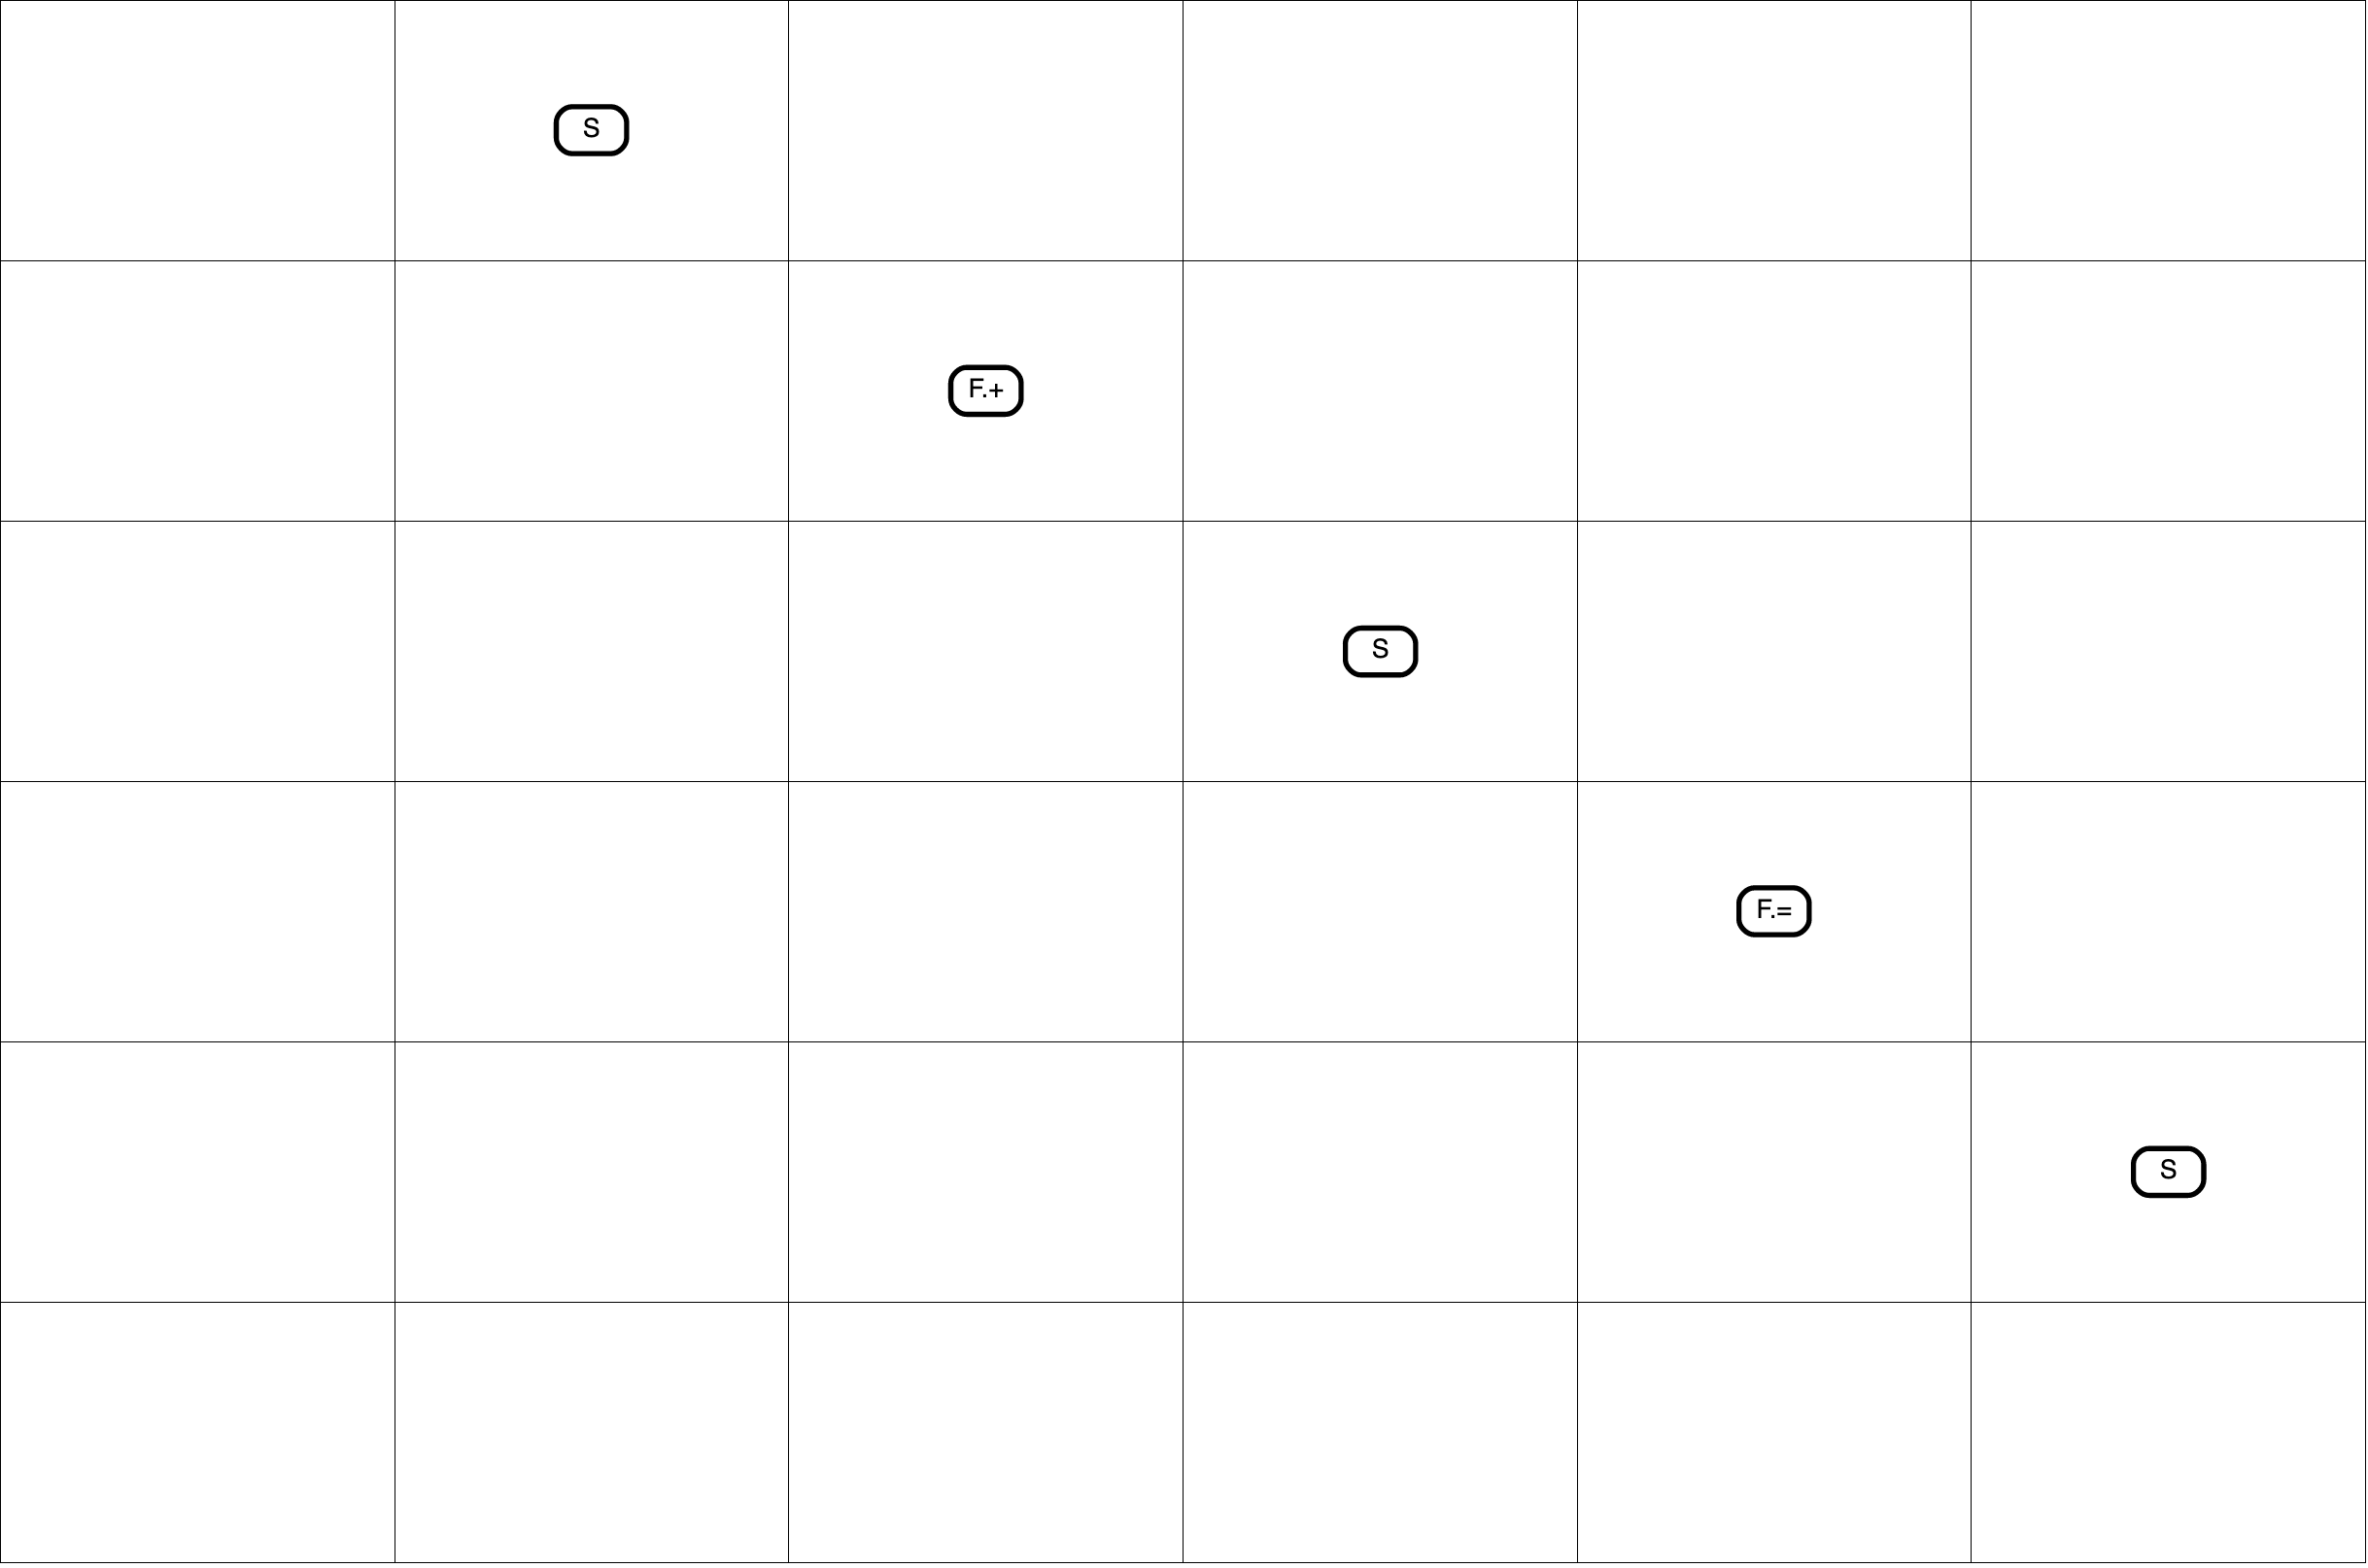
\includegraphics[width=2cm]{../figures/parse1.png}
%    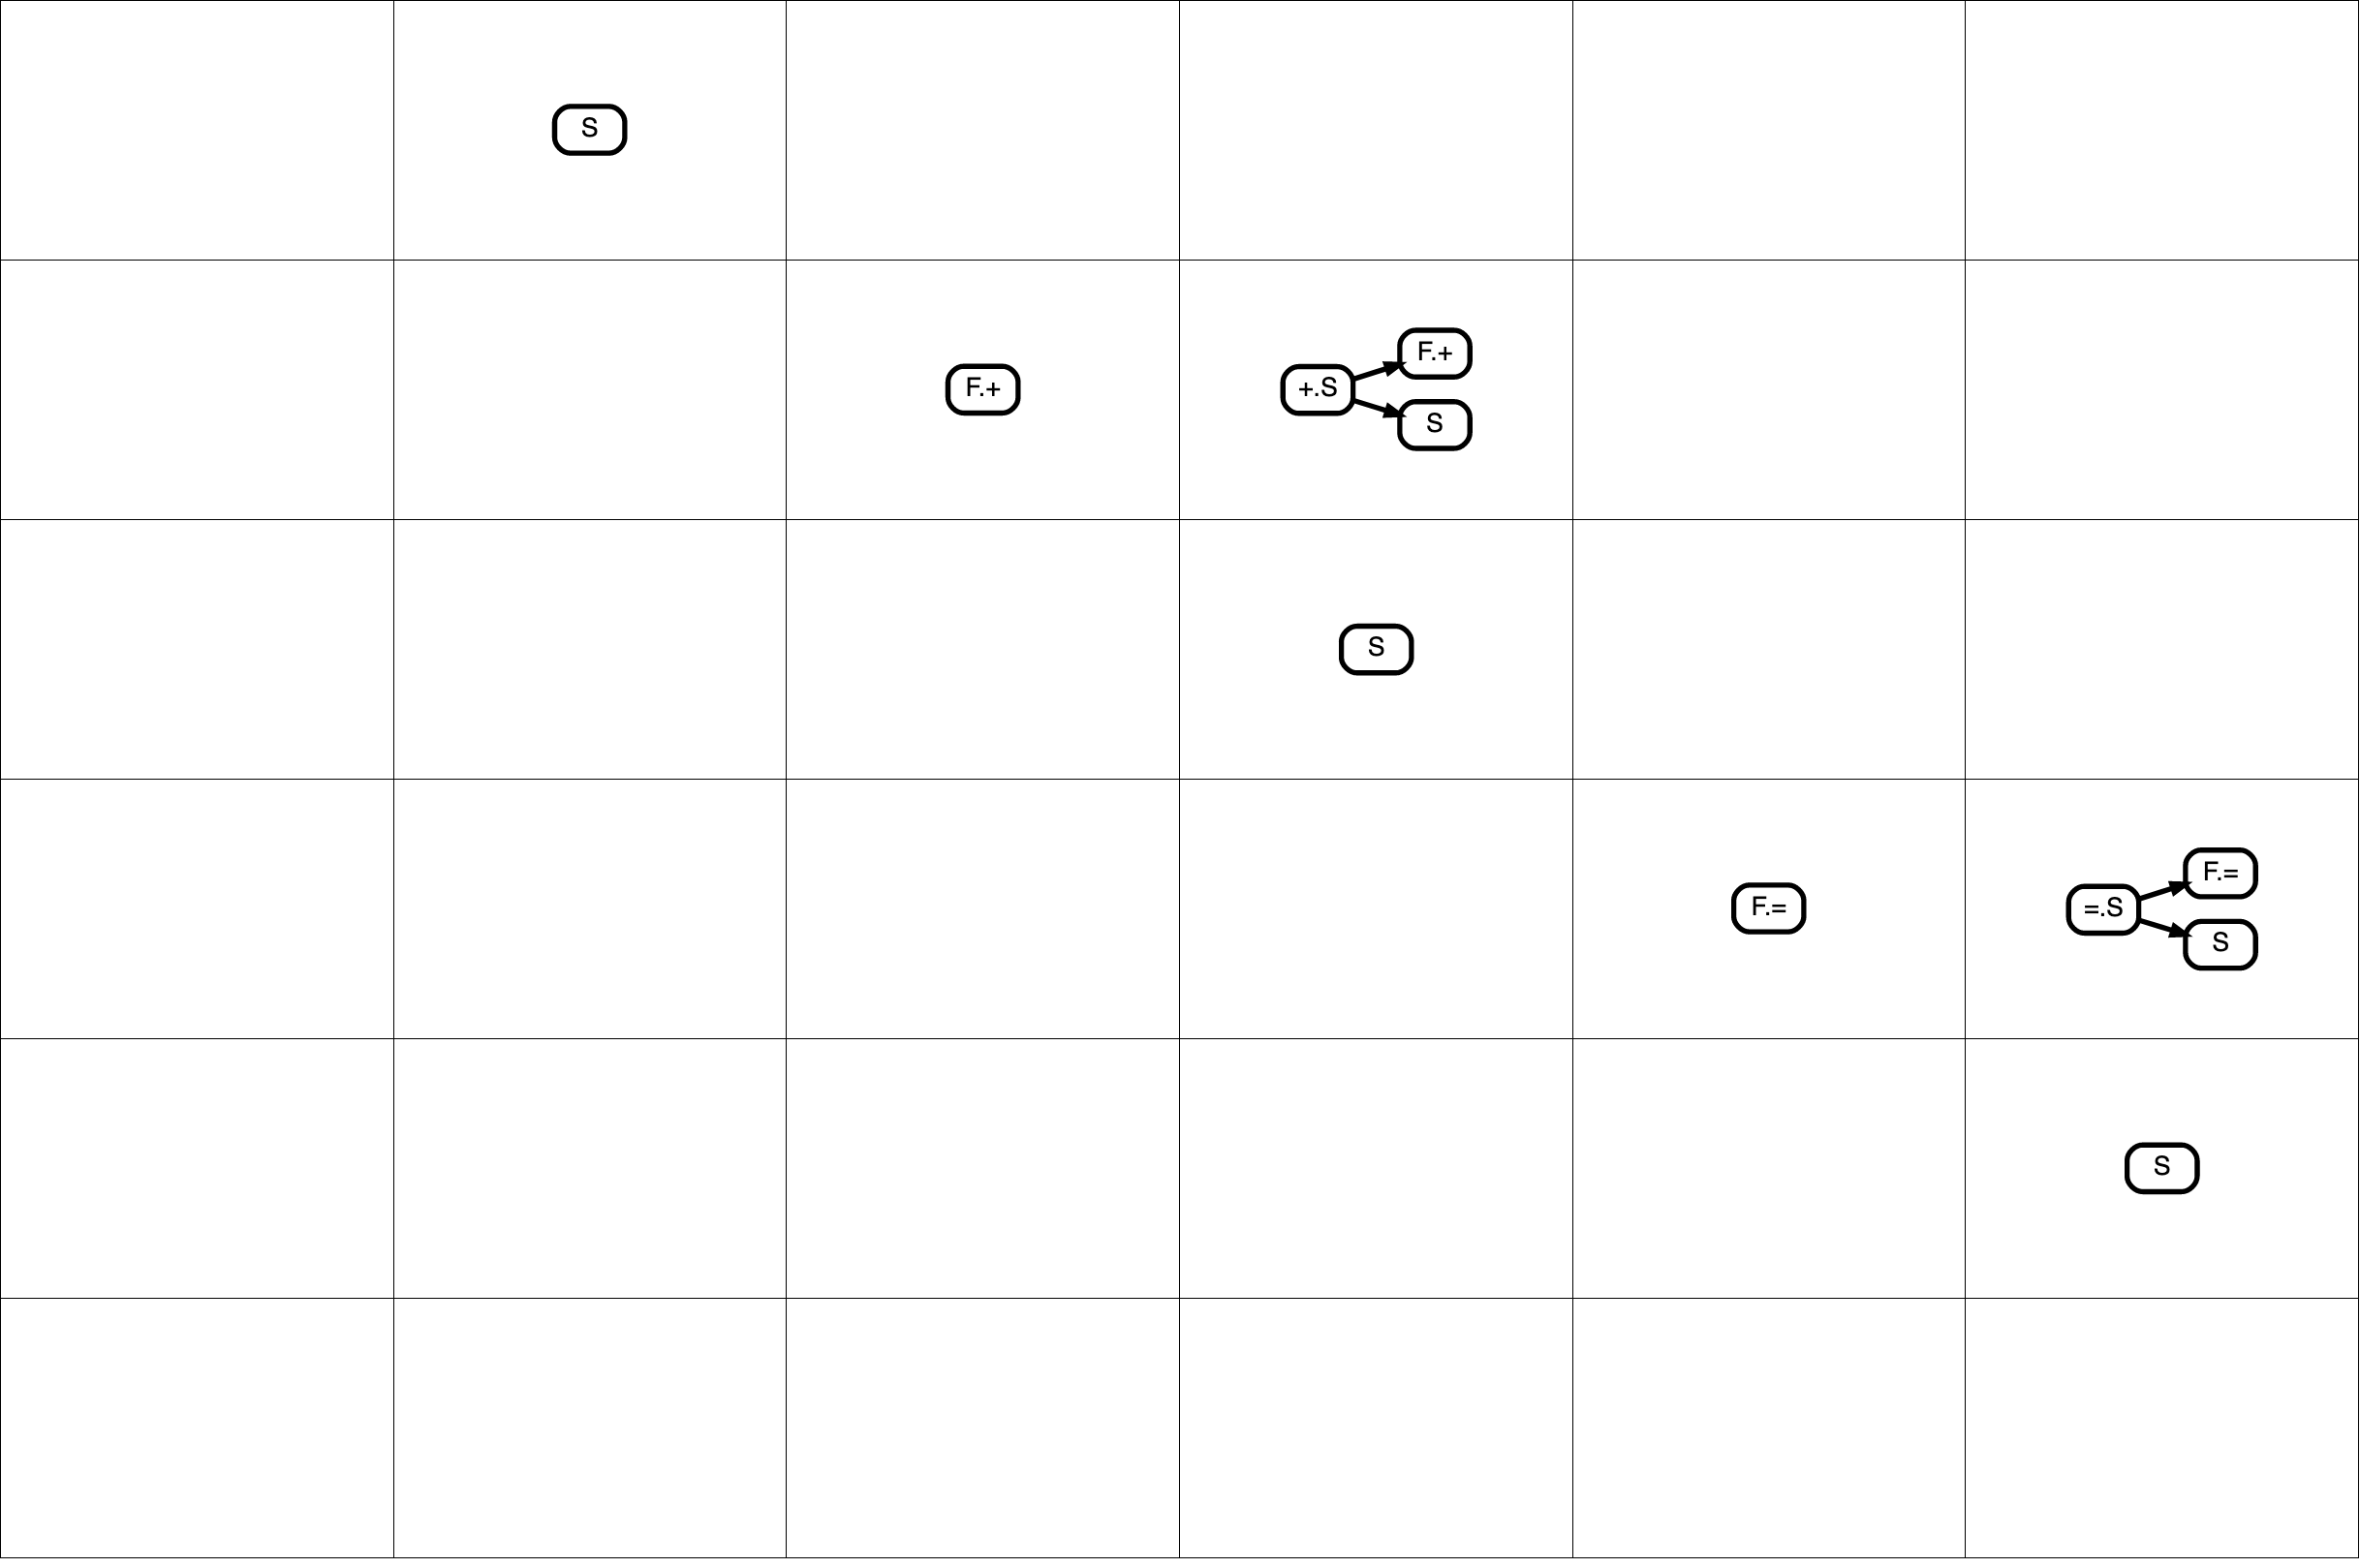
\includegraphics[width=2cm]{../figures/parse2.png}
%    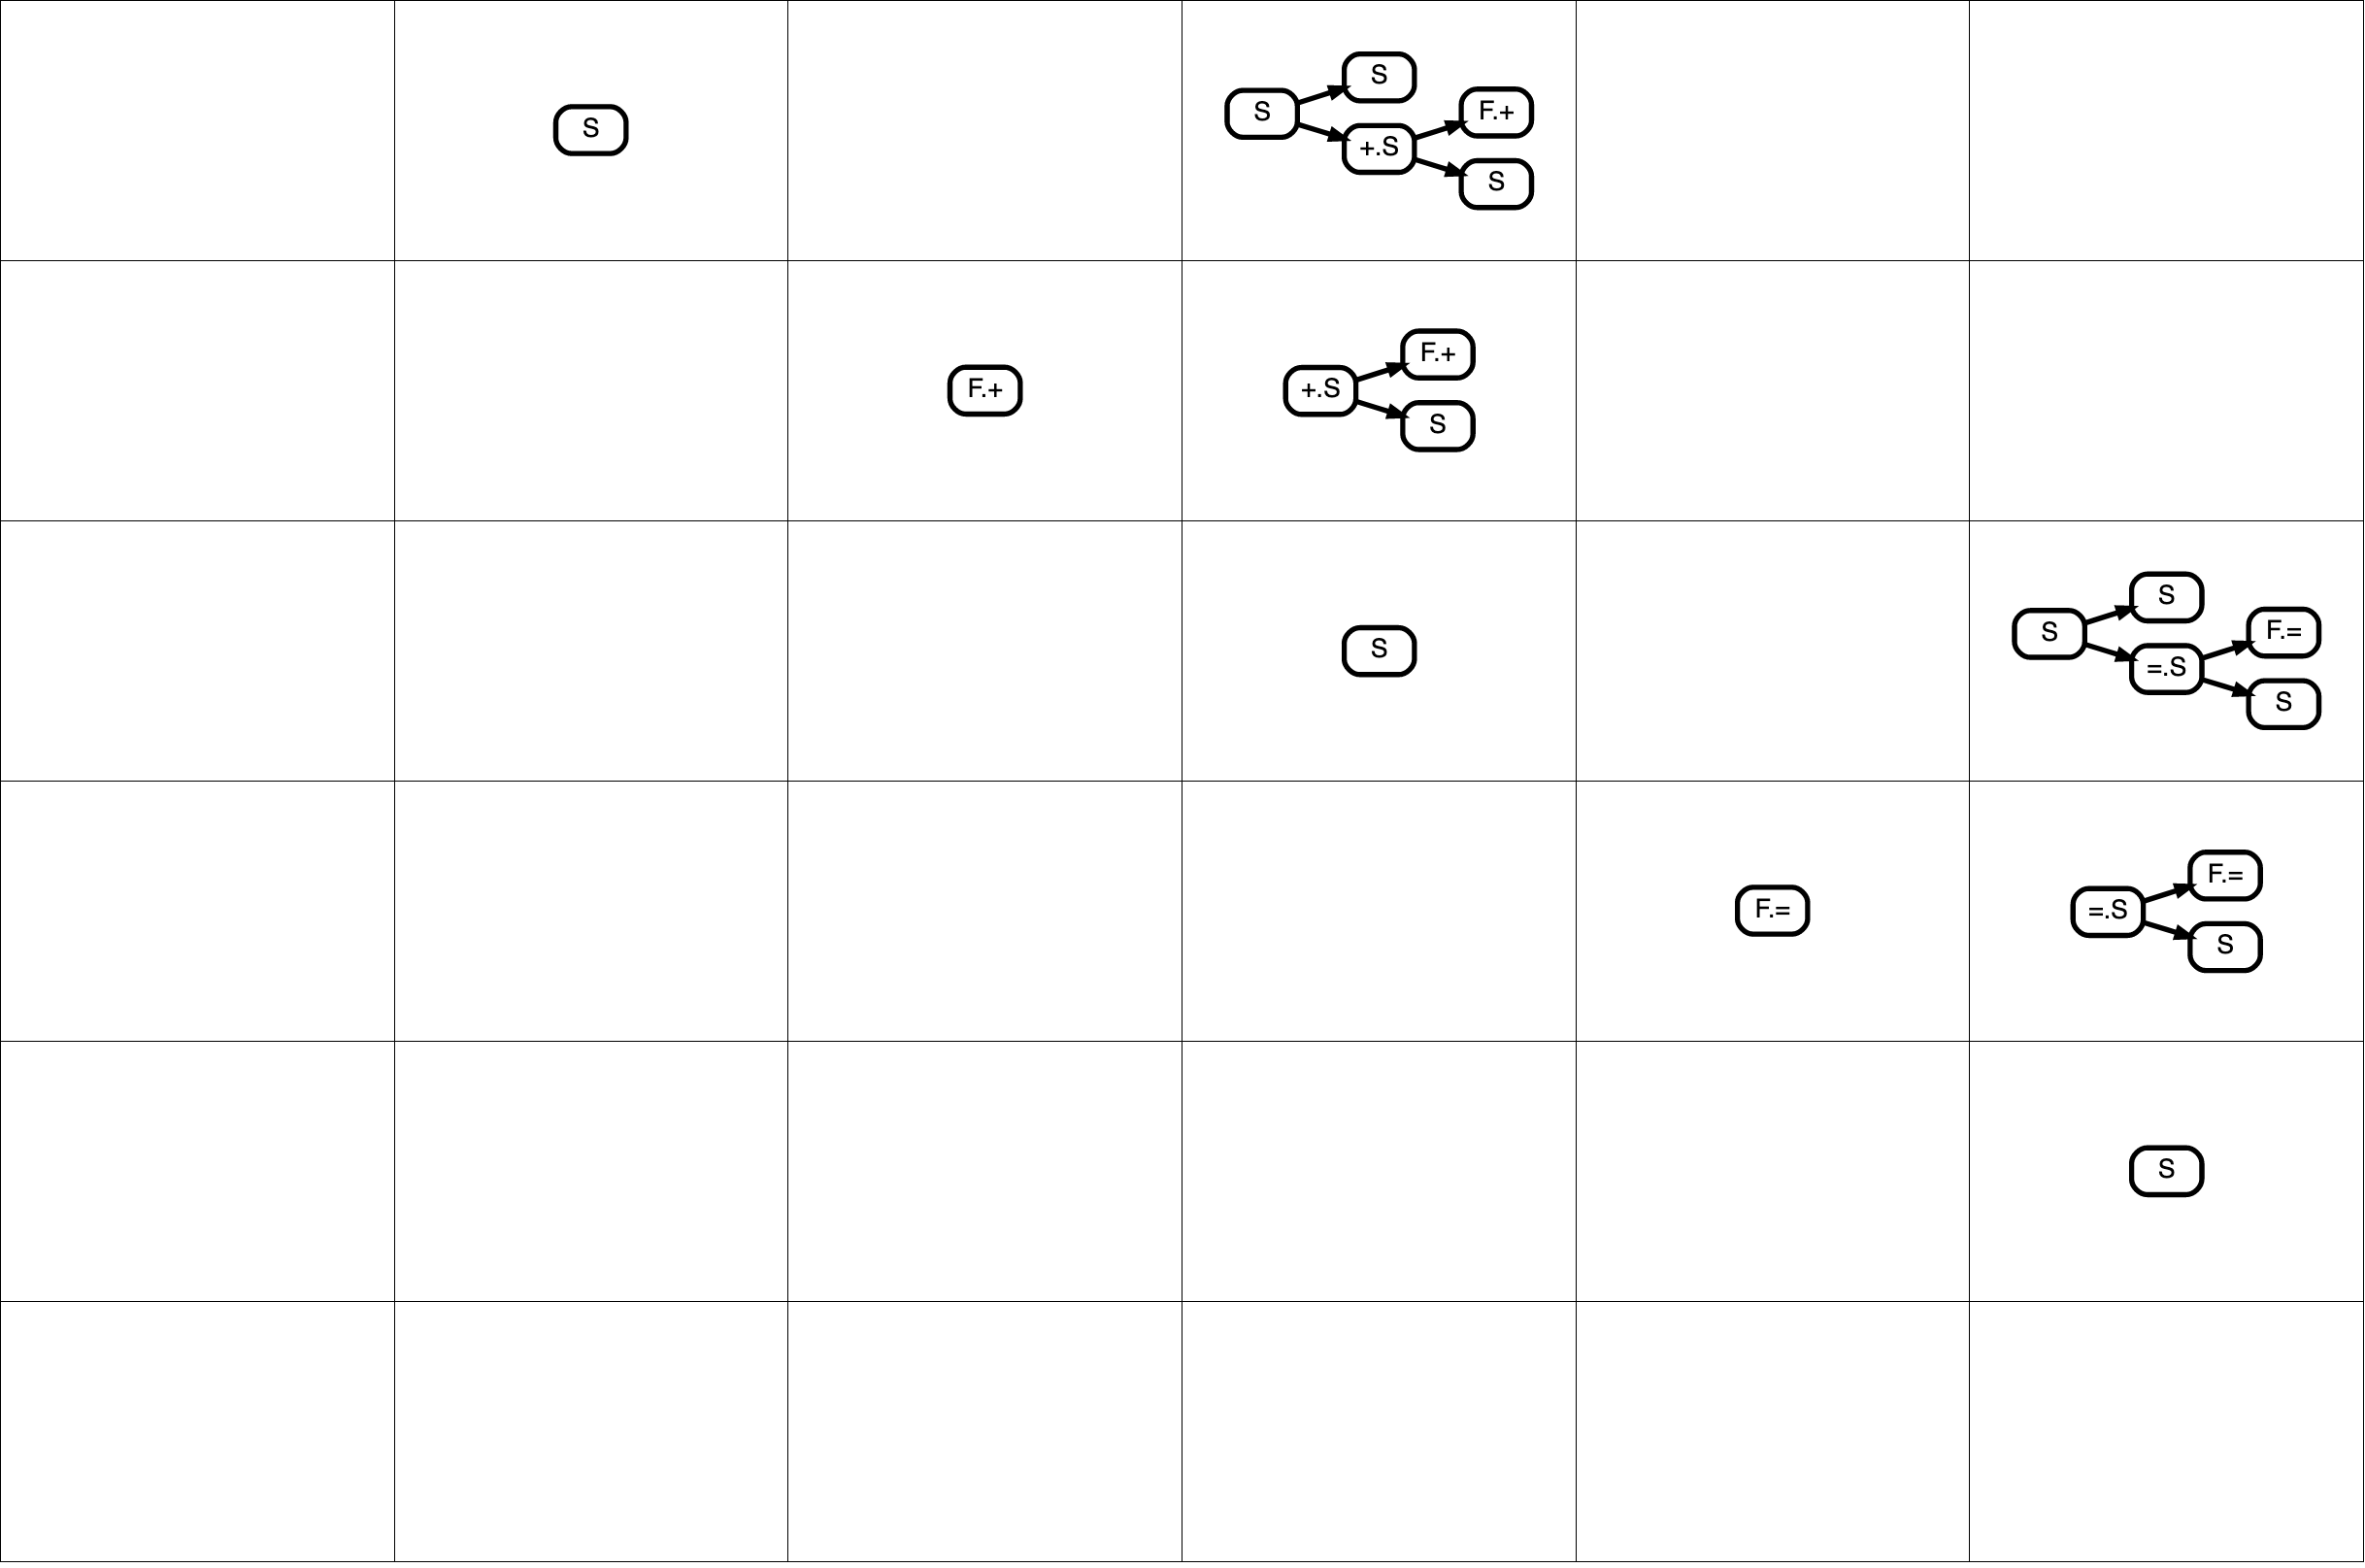
\includegraphics[width=2cm]{../figures/parse3.png}
%    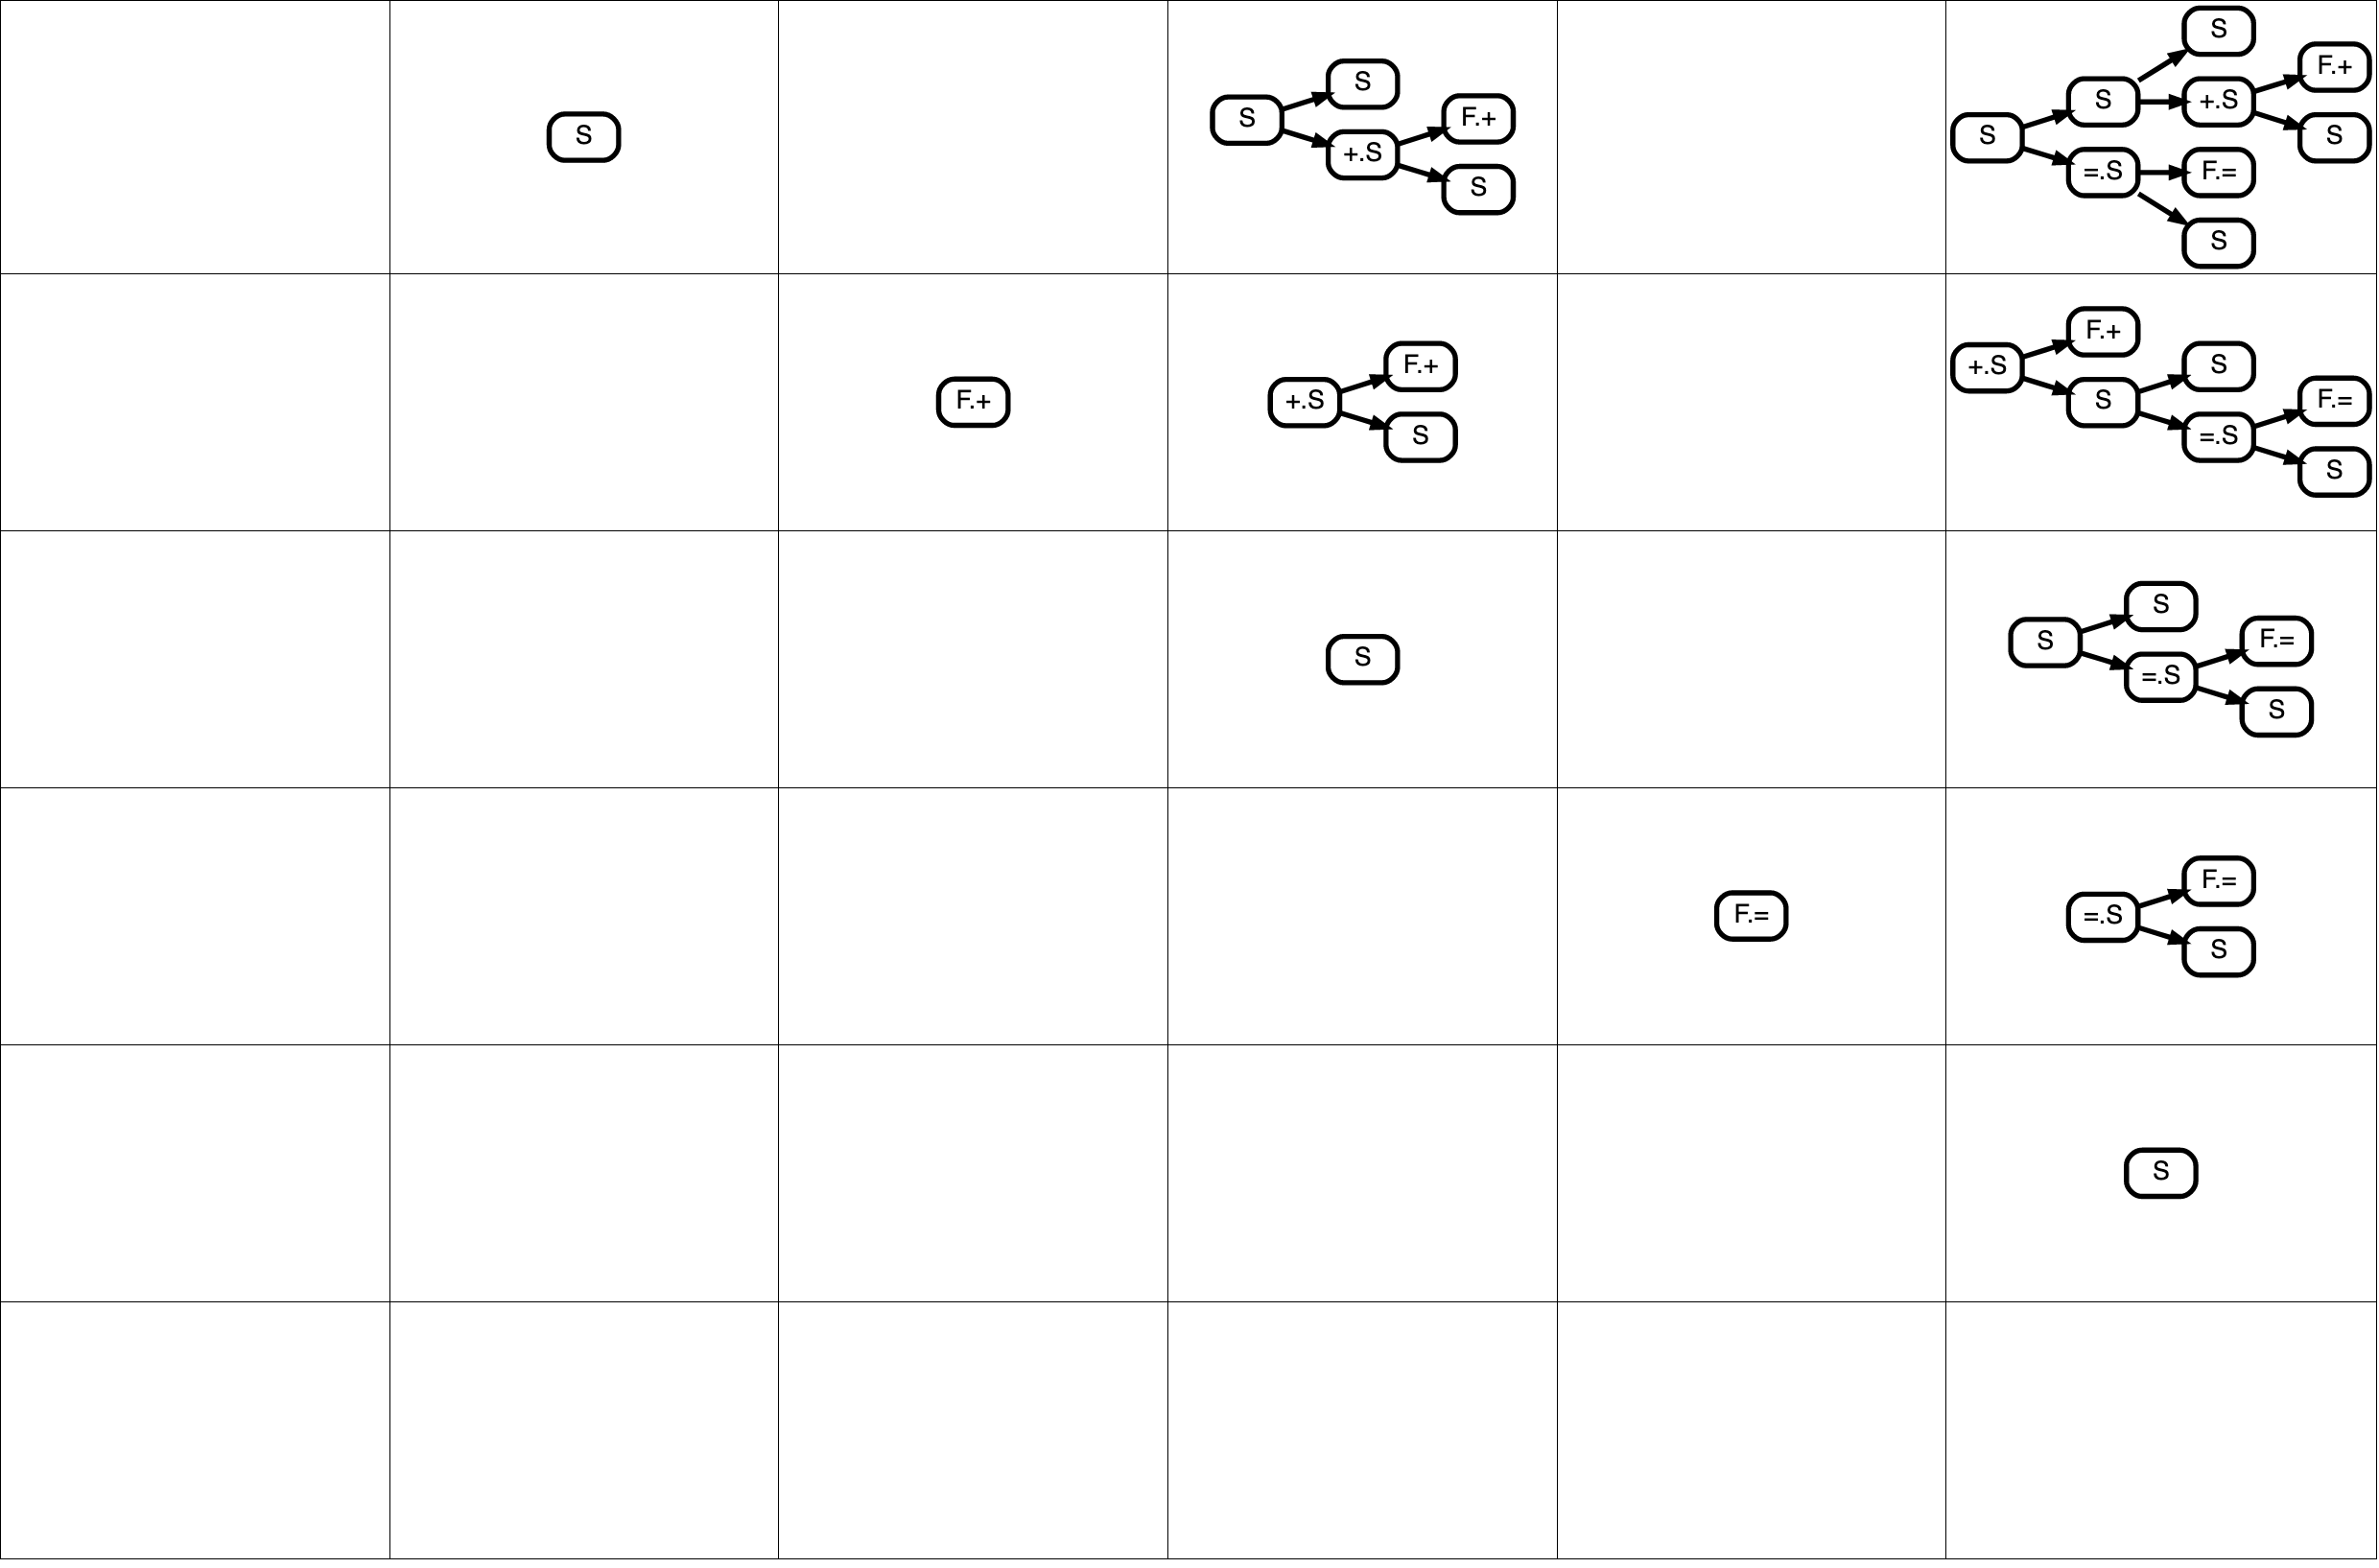
\includegraphics[width=2cm]{../figures/parse4.png}
%\end{figure}

\newcommand\ddd{\Ddots}
\newcommand\vdd{\Vdots}
\newcommand\cdd{\Cdots}
\newcommand\lds{\ldots}
\newcommand\vno{\varnothing}
\newcommand{\ts}[1]{\textsuperscript{#1}}
\newcommand\non{1\ts{st}}
\newcommand\ntw{2\ts{nd}}
\newcommand\nth{3\ts{rd}}
\newcommand\nfo{4\ts{th}}
\newcommand\nfi{5\ts{th}}
\newcommand\nsi{6\ts{th}}
\newcommand\nse{7\ts{th}}
\newcommand{\vs}[1]{\{V\}_{\sigma_{#1}}}
\newcommand\rcr{\rowcolor{black!15}}
\newcommand\rcw{\rowcolor{white}}
\newcommand\pcd{\cdot}
\newcommand\pcp{\phantom\cdot}
\newcommand\ppp{\phantom{\nse}}

\begin{figure}[H]
\[
  \mathbf{M}^* = \begin{pNiceArray}{>{\strut}ccccccc}[margin, extra-margin=2pt,colortbl-like, xdots/line-style=loosely dotted]
    \vno & \rcr \vs{1} &  \mathcal{L}_{1,3} & \mathcal{L}_{1,3} & \rcw \mathcal{V}_{1,4} & \cdd & \mathcal{V}_{1,n} \\
    \vdd & \ddd        &  \rcr\vs{2}        & \mathcal{L}_{2,3} & \rcw\vdd               &      & \vdd \\
         &             &                    & \rcr\vs{3}        & \rcw                   &      & \\
         &             &                    &                   & \mathcal{V}_{4,4}      &      & \\
         &             &                    &                   &                        & \ddd & \\
         &             &                    &                   &                        &      & \mathcal{V}_{n,n} \\
    \vno & \cdd        &                    &                   &                        &      & \vno
  \end{pNiceArray}
\]
\end{figure}

\noindent Depicted above is a SAT tensor representing \hlgray{$\sigma_1\:\sigma_2\:\sigma_3$}$\:\_\:\ldots\:\_$ where shaded regions demarcate known bitvector literals $\mathcal{L}_{r,c}$ (i.e., representing established nonterminal forests) and unshaded regions correspond to bitvector variables $\mathcal{V}_{r,c}$ (i.e., representing seeded nonterminal forests to be grown). Since $\mathcal{L}_{r,c}$ are fixed, we precompute them outside the SAT solver.

\subsection{Deletion, substitution, and insertion}\label{sec:dsi}

Deletion, substitution and insertion can be simulated by first adding a left- and right- $\varepsilon$-production to each unit production:\vspace{5pt}

\begin{prooftree}
    \AxiomC{$\Gamma \vdash \varepsilon \in \Sigma$}
    \RightLabel{$\varepsilon\textsc{-dup}$}
    \UnaryInfC{$\Gamma \vdash (\varepsilon^+ \rightarrow \varepsilon \mid \varepsilon^+\:\varepsilon^+) \in P$}
\end{prooftree}

\begin{prooftree}
    \AxiomC{$\Gamma \vdash (A \rightarrow B) \in P$}
    \RightLabel{$\varepsilon^+\textsc{-int}$}
    \UnaryInfC{$\Gamma \vdash (A \rightarrow B\:\varepsilon^+ \mid \varepsilon^+\:B \mid B) \in P$}
\end{prooftree}

\vspace{5pt}
\noindent To generate the sketch templates, we substitute two holes at an index-to-be-repaired, $H(\sigma, i) = \sigma_{1\ldots i-1}\:\texttt{\_ \_}\:\sigma_{i+1\ldots n}$, then invoke the SAT solver. Five outcomes are then possible:

\begin{align}
&\sigma_{1}\ldots\sigma_{i-1}\:\text{\hlred{$\gamma_1$}\hlred{$\gamma_2$}}\:\sigma_{i+1}\ldots\sigma_{n}, \gamma_{1, 2} = \varepsilon\label{eq:del}\\
&\sigma_{1}\ldots \sigma_{i-1}\:\text{\hlorange{$\gamma_1$}\hlred{$\gamma_2$}}\:\sigma_{i+1}\ldots \sigma_{n}, \gamma_1 \neq \sigma_i, \gamma_2 = \varepsilon\label{eq:sub1}\\
&\sigma_{1}\ldots \sigma_{i-1}\:\text{\hlred{$\gamma_1$}\hlorange{$\gamma_2$}}\:\sigma_{i+1}\ldots \sigma_{n}, \gamma_1 = \varepsilon, \gamma_2 \neq \sigma_i\label{eq:sub2}\\
&\sigma_{1}\ldots\sigma_{i-1}\: \text{\hlorange{$\gamma_1$}\hlgreen{$\gamma_2$}}\:\sigma_{i+1}\ldots\sigma_{n}, \gamma_1 = \sigma_i, \gamma_2 \neq \varepsilon\label{eq:ins1}\\
&\sigma_{1}\ldots\sigma_{i-1}\: \text{\hlgreen{$\gamma_1$}\hlorange{$\gamma_2$}}\:\sigma_{i+1}\ldots\sigma_{n}, \gamma_1 \notin \{\varepsilon, \sigma_i\}, \gamma_2 = \sigma_i\label{eq:ins2}
\end{align}

\noindent Eq.~(\ref{eq:del}) corresponds to deletion, Eqs.~(\ref{eq:sub1},~\ref{eq:sub2}) correspond to substitution, and Eqs.~(\ref{eq:ins1},~\ref{eq:ins2}) correspond to insertion. This procedure is repeated for all indices in the replacement set. The solutions returned by the SAT solver will be strictly equivalent to handling each edit operation as separate cases.

\section{Error Recovery}\label{sec:error}

Unlike classical parsers which need special care to recover from errors, if the input string does not parse, Tidyparse can return partial subtrees. If no solution exists, the upper triangular entries will appear as a jagged-shaped ridge whose peaks represent the roots of parsable ASTs. These provide a natural debugging environment to aid the repair process.

\begin{tidyinput}
true and true ! and false or true ! true and false(*@\caret{ }@*)
\end{tidyinput}

\begin{verbatim}
 Parseable subtrees (3 leaves / 2 branches):
\end{verbatim}
\noindent\hspace{0.64cm}\emoji{herb}\hspace{1.70cm}\emoji{herb}\hspace{1.98cm}\emoji{herb}\vspace{-5pt}
\begin{verbatim}
    └── ! [3]   └── and [4]   └── or [6]
\end{verbatim}
\hspace{0.63cm}\emoji{herb}\hspace{3.4cm}\emoji{herb}\vspace{-5pt}
\begin{verbatim}
    └── S [0..2]          └── S [8..11]
        ├── true [0]          ├── S [8..9]
        ├── and [1]           │   ├── ! [8]
        └── true [2]          │   └── true [9]
                              ├── and [10]
                              └── false [11]
\end{verbatim}

\noindent These branches correspond to peaks on the upper triangular (UT) matrix ridge. As depicted in Fig.~\ref{fig:peaks}, we traverse the peaks by decreasing elevation to collect partial AST branches.

\begin{figure}[H]
\[
  \setcounter{MaxMatrixCols}{30}
  \begin{NiceMatrix}
                 & \nse & \nsi & \nfi & \nfo & \nth & \ntw & \non & \ppp & \ppp \\
                 &      & \ddd & \ddd & \ddd & \ddd & \ddd & \ddd & \ddd & \ppp \\
\{V\}_{\sigma_1} & \cdd &      & A    &      &      &      &      &      & \ppp \\
\varnothing      & \ddd &  T_A & \vdd &      &      &      &      &      & \ppp \\
\vdd             & \ddd &      & \pcd & \cdd &      & B    &      &      & \ppp \\
                 &      &      &      &      & T_B  & \vdd &      &      & \ppp \\
                 &      &      &      &      &      & \pcd & \cdd &      & C    \\
                 &      &      &      &      &      &      &      & T_C  & \vdd \\
                 &      &      &      &      &      &      & \text{\emoji{cross-mark}} &      & \\
                 &      &      &      &      &      &      &      &      & \\
                 &      &      &      &      &      &      &      &      & \\
                 &      &      &      &      &      &      &      & \ppp & \{V\}_{\sigma_n} \\
\varnothing      & \cdd &      &      &      &      &      &      & \varnothing &
  \end{NiceMatrix}
\]\caption{Peaks along the UT matrix ridge correspond to maximally parseable substrings. By recursing over upper diagonals of decreasing elevation and discarding all subtrees that fall under the shadow of another's canopy, we can recover the partial subtrees. The example depicted above contains three such branches, rooted at nonterminals $C, B, A$.}\label{fig:peaks}
\end{figure}

\section{Tree Denormalization}

% https://www.ling.upenn.edu/advice/latex/qtree/qtreenotes.pdf
% https://cpb-us-w2.wpmucdn.com/campuspress.yale.edu/dist/0/119/files/2014/12/sec-10.17-drawing-arrows-2ek9r2b.pdf

Our parser emits a binary forest consisting of parse trees for the candidate string according to the CNF grammar, however this forest contains many so-called \textit{Krummholz}, or \textit{flag trees}, often found clinging to windy ridges and mountainsides.

\begin{figure}[H]
\resizebox{.50\textwidth}{!}{
\begin{tabular}{ll}
    \Tree [.\texttt{S} \tikz\node(v1){\texttt{true}} [.$\ccancel{\texttt{and.S}}$ \tikz\node(v3){\texttt{and}} [.\texttt{S} \tikz\node(v5){\texttt{(}} [.$\ccancel{\texttt{S.)}}$ [.\texttt{S} \tikz\node(v9){\texttt{false}} [.$\ccancel{\texttt{or.S}}$ \tikz\node(v11){\texttt{or}} [.\texttt{S} \texttt{!} \texttt{true} ] ] ] \tikz\node(v7){\texttt{)}} ] ] ] ]
%    \Tree [.S [.NP John ] [.VP [.\tikz\node(v1){V}; sleeps ] ] ]
    \hspace{-2cm}
    &
    \Tree [.\texttt{S} \tikz\node(v2){\texttt{true}} \tikz\node(v4){\texttt{and}} [.\texttt{S} \tikz\node(v6){\texttt{(}} [.\texttt{S} \tikz\node(v10){\texttt{false}} \tikz\node(v12){\texttt{or}} [.\texttt{S} \texttt{!} \texttt{true} ] ] \tikz\node(v8){\texttt{)}} ] ]\\\\
%    \Tree [.\tikz\node(v2){V}; [.\tikz\node(v3){V}; ] [.Adv {a lot} ] ]
    \hspace{1cm}\huge{Pre-Denormalization} & \hspace{3cm}\huge{Post-Denormalization}
\end{tabular}
\begin{tikzpicture}[overlay]
%    \draw [red,dashed,-stealth] (v1) to[bend left] (v2);
    \draw [red,dashed,-stealth] (v3) to[bend left] (v4);
%    \draw [red,dashed,-stealth] (v5) to[bend left] (v6);
    \draw [red,dashed,-stealth] (v7) to[bend left] (v8);
%    \draw [red,dashed,-stealth] (v9) to[bend right] (v10);
    \draw [red,dashed,-stealth] (v11) to[bend right] (v12);
\end{tikzpicture}
}
%    \caption{Result of applying Algorithm~\ref{alg:cap} to the tree obtained by parsing the string: \texttt{true and ( false or ! true )}.}
\end{figure}\vspace{-10pt}
\begin{algorithm}
    \caption{Rewrite procedure for tree denormalization}\label{alg:cap}
    \begin{algorithmic}
        \Procedure{Denormalize}{\texttt{t: Tree}}
            \State $\texttt{stems} \leftarrow \{\:\textsc{Denormalize}(\texttt{c}) \mid \texttt{c} \in \texttt{t.children}\:\}$
            \If{$\texttt{t.root} \in V_{\mathcal{G}'} \setminus V_{\mathcal{G}}$}
                \State \textbf{return } \texttt{stems} \Comment{Drop synthetic nonterminals.}
            \Else\Comment{Graft the denormalized children on root.}
                \State \textbf{return } $\{\:\texttt{Tree(root, stems)}\:\}$
            \EndIf
        \EndProcedure
    \end{algorithmic}
\end{algorithm}

\noindent To recover a parse tree congruent with the user-specified grammar, we prune all synthetic nodes and graft their stems onto the grandparent via a simple recursive procedure (Alg.~\ref{alg:cap}).%, which is used to denormalize both complete and partial ASTs (cf. \S~\ref{sec:error}) alike.

\section{Realtime Error Correction}\label{sec:holes}

Now that we have a reliable method to fix \textit{localized} errors, $S: \mathcal{G} \times (\Sigma\cup\{\varepsilon, \texttt{\_}\})^n \rightarrow \{\Sigma^n\}\subseteq \mathcal{L}_\mathcal{G}$, given an input string, $\Sigma^n$, where should we put the holes? Assuming $k$ holes, there are ${n \choose k}$ possible hole configurations (HCs), each with $(|\Sigma| + 1)^{2k}$ possible repairs (before parsing, cf. Eqs.~\ref{eq:del}-\ref{eq:ins2}). In practice, depending on $n$ and $k$, this space can be intractable to search through exhaustively, so to facilitate real-time assistance we prioritize likely repairs according to an eight-step procedure:

\begin{enumerate}
  \item Fetch the most recent CFG and string from the editor.
  \item Exclude parsable substrings from hollowing.
  \item Lazily enumerate all HCs of increasing length.
  \item Sample HCs without replacement using Eq.~\ref{eq:ergo}.
  \item Prioritize HCs first by distance to caret index, then by Earthmover's distance to a set of suspicious indices.$^*$
  \item Translate HCs to sketch templates using~\S\ref{sec:dsi}.
  \item Feed sketch templates to an incremental SAT solver.
  \item Decode and rerank models by Levenshtein distance.
\end{enumerate}

\noindent $^*$ These locations can be supplied by local edit history or using tokenwise perplexity from a neural language model. Once a new repair is discovered, it is immediately displayed. Incoming keystrokes interrupt and reset the solving process.

\section{Practical Example}

Tidyparse requires a grammar -- this can be either provided by the user or ingested from a BNF-like specification. The following is a slightly more complex grammar, designed to resemble a more realistic use case:

\begin{tidyinput}
S -> A | V | ( X , X ) | X X | ( X )
A -> Fun | F | L | L in X
Fun -> fun V (*@`@*)->(*@`@*) X
F -> if X then X else X
L -> let V = X | let rec V = X
V -> Vexp | ( Vexp ) | Vexp Vexp
Vexp -> VarName | FunName | Vexp VO Vexp
Vexp -> ( VarName , VarName ) | Vexp Vexp
VarName -> a | b | c | d | e | ... | z
FunName -> foldright | map | filter
VO ->  + | - | * | / | > | = | < | (*@`@*)||(*@`@*) | &&
---
let curry f = ( fun x y -> f ( _ _ _(*@\caret{ }@*)) )
\end{tidyinput}
\begin{tidyoutput}
let curry f = ( fun x y -> f ( (*@\hlorange{<X>}@*) ) )
let curry f = ( fun x y -> f ( (*@\hlorange{<FunName>}@*) ) )
let curry f = ( fun x y -> f ( (*@\hlorange{curry}@*) (*@\hlorange{<X>}@*) ) )
...
\end{tidyoutput}

\subsection{Grammar Assistance}

Tidyparse uses a CFG to parse the CFG, so it can provide assistance while the user is designing the CFG. For example, if the CFG does not parse, it will suggest possible fixes. In the future, we intend to use this functionality to perform example-based codesign and grammar induction.

\begin{tidyinput}
B -> true | false | (*@\caret{ }@*)
\end{tidyinput}
\begin{tidyoutput}
B -> true | false (*@\hlred{ }@*)
B -> true | false (*@\hlorange{<RHS>}@*)
B -> true | false | (*@\hlgreen{<RHS>}@*)
...
\end{tidyoutput}

\subsection{Interactive Nonterminal Expansion}

Users can interactively build up a complex expression by placing the caret over a placeholder they wish to expand,

\begin{tidyinput}
if <(*@\caret{V}@*)exp> X then <Vexp> else <Vexp>
\end{tidyinput}

\noindent then invoking Tidyparse by pressing \keys{\ctrl + \SPACE}, to receive a list of expressions consistient with the grammar:

\begin{tidyoutput}
if (*@\hlorange{map}@*) X then <Vexp> else <Vexp>
if (*@\hlorange{uncurry}@*) X then <Vexp> else <Vexp>
if (*@\hlorange{foldright}@*) X then <Vexp> else <Vexp>
...
\end{tidyoutput}

%There are some more examples too.
%
%The line between parsing and computation is blurry.

\pagebreak
\section{Latency Benchmark}

In the following benchmarks, we measure the wall clock time required to synthesize solutions to length-50 strings sampled from various Dyck languages, where Dyck-n is the Dyck language containing n types of balanced parentheses.

\begin{tidyinput}
D1 -> () | ( D1 ) | D1 D1
D2 -> D1 | [ ] | ( D2 ) | [ D2 ] | D2 D2
D3 -> D2 | { } | ( D3 ) | [ D3 ] | { D3 } | D3 D3
\end{tidyinput}

\noindent In the first experiment, we sample a random valid string $\sigma \sim \Sigma^{50} \cap \mathcal{L}_{\text{Dyck-n}}$, then replace a fixed number tokens with holes and measure the average time taken to decode ten syntactically-admissible repairs across 100 trial runs.

\begin{tikzpicture}
  \begin{axis}[
      width=8.3cm,
    title={\hspace{-1cm}\textbf{Error correction time with known locations}},
    ybar,
    bar width=4pt,
    xlabel={Number of holes},
    ylabel={ms to synthesize 10 repairs},
    xtick=data,
    axis x line*=bottom,
    axis y line*=left,
    ytick pos=left,
    xticklabels from table={\loctimings}{holes},
    ymajorgrids,
    legend pos=north west,
    error bars/y dir=both,
    error bars/y explicit
  ]
    \addplot table [x expr=\coordindex, y=d1, y error=d1err]{\loctimings};
    \addplot table [x expr=\coordindex, y=d2, y error=d2err]{\loctimings};
    \addplot table [x expr=\coordindex, y=d3, y error=d3err]{\loctimings};
    \addplot table [x expr=\coordindex, y=d4, y error=d4err]{\loctimings};
    \legend{Dyck-1, Dyck-2, Dyck-3, Dyck-4}
  \end{axis}
\end{tikzpicture}

\noindent In the second experiment, we sample a random valid string as before, but delete p tokens at random and rather than provide the location(s), ask our model to solve for both the location(s) and repair by sampling uniformly from all n-token HCs, then measure the total time required to decode the first admissible repair. Note the the logarithmic scale on the y-axis.

\begin{tikzpicture}
    \begin{axis}[
        width=8.3cm,
        height=6.6cm,
        title={\hspace{-1cm}\textbf{Error correction time with unknown locations}},
        ybar,
        bar width=20pt,
        xlabel={Number of errors},
        ylabel={ms to synthesize 1 repair},
        xtick=data,
        axis x line*=bottom,
        axis y line*=left,
        enlarge x limits={abs=0.5},
        ymode=log,
        ytick pos=left,
        xticklabels from table={\unloctimings}{errors},
        ymajorgrids,
        legend pos=north west,
        error bars/y dir=both,
        error bars/y explicit
    ]
        \addplot table [x expr=\coordindex, y=d1]{\unloctimings};
        \addplot table [x expr=\coordindex, y=d2]{\unloctimings};
        \addplot table [x expr=\coordindex, y=d3]{\unloctimings};
        \legend{Dyck-1, Dyck-2, Dyck-3}
    \end{axis}
\end{tikzpicture}

\section{Discussion}

While error correction with a few errors is tolerable, latency can vary depending on many factors including string length and grammar size. If errors are known to be concentrated in specific locations, such as the beginning or end of a string, then latency is typically below 500ms. Should errors occur uniformly at random, admissible repairs can take longer to discover, however these scenarios are unusual in our experience. We observe that errors are typically concentrated nearby historical edit locations, which can be retrieved from the IDE or version control. Further optimizations that reduce the total number of repairs checked are possible by eliminating improbable sketch templates.

Tidyparse in its current form has a number of technical shortcomings: firstly it does not incorporate any neural language modeling technology at present, an omission we hope to address in the near future. Training a language model to predict likely repair locations and rank admissible results could lead to lower overall latency and more natural repairs.

Secondly, our current method generates sketch templates using a na\"ive enumerative search, feeding them individually to the SAT solver, which has the tendency to duplicate prior work and introduces unnecessary thrashing. Considering recent extensions of Boolean matrix-based parsing to linear context-free rewriting systems (LCFRS)~\cite{cohen2016parsing}, it may be feasible to search through these edits within the SAT solver, leading to yet unrealized and possibly significant speedups.

Lastly and perhaps most significantly, Tidyparse does not incorporate any semantic constraints, so its repairs while syntactically admissible, are not guaranteed to be semantically valid. We note however, that it is possible to encode type-based semantic constraints into the solver and intend to explore this direction more fully in future work.

Although not intended to be a dedicated parser and we make no attempt to rigorously compare parsing latency, parsing valid strings with Tidyparse is typically competitive with classical parsing methods. Our primary motivation is to facilitate the usability and explainability of parsing with errors. We envision three primary use cases: (1) helping novice programmers become more quickly familiar with a new programming language (2) autocorrecting common typos among proficient but forgetful programmers and (3) as a prototyping tool for PL educators and designers.

Featuring a grammar editor and built-in SAT solver, Tidyparse helps developers navigate the language design space, visualize syntax trees, debug parsing errors and quickly generate simple examples and counterexamples for testing. Although the algorithm may seem esoteric at first glance, in our experience it is much more interpretable than classical parsers, which exhibit poor error-recovery and diagnostics.

\section{Conclusion}

Tidyparse accepts a CFG and a string to parse. If the string is valid, it returns the parse forest, otherwise, it returns a set of repairs, ordered by their Levenshtein edit distance to the invalid string. Our method compiles each CFG and candidate string onto a matrix dynamical system using an extended version of Valiant's construction and solves for its fixedpoints using an incremental SAT solver. This approach to parsing has many advantages, enabling us to repair syntax errors, correct typos and generate parse trees for incomplete strings. By allowing the string to contain holes, repairs can contain either concrete tokens or nonterminals, which can be manually expanded by the user or a neural-guided search procedure. From a theoretical standpoint, this technique is particularly amenable to neural program synthesis and repair, naturally integrating with the masked-language-modeling task (MLM) used by transformer-based neural language models.

From a practical standpoint, we have implemented our approach as an IDE plugin and demonstrated its viability as a tool for live programming. Tidyparse is capable of generating repairs for invalid code in a range of toy languages. We plan to continue expanding its grammar and autocorrection functionality to cover a broader range of languages and hope to conduct a more thorough user study to validate its effectiveness in the near future. Further examples can be found at our GitHub repository: \url{https://github.com/breandan/tidyparse}
%\begin{itemize}
%\item Error correction.
%\item Program repair.
%\item Program synthesis.
%\item Parsing with holes.
%\item Naturally integrates with masked language model (MLM)-based neural program repair.
%\item Parsing with natural error recovery.
%\item Helps to facilitate language learning.
%\item GPU acceleration.
%\end{itemize}

\section{Acknowledgements}
The first author would like to thank his co-advisor Xujie Si for providing many helpful suggestions during the development of this project, including the optimized fixpoint, test cases, and tree denomalization procedure, Zhixin Xiong for contributing the OCaml grammar and collaborator Nghi Bui at FPT Software for early feedback on the IDE plugin.
\bibliography{../bib/acmart}
\end{document}